% Options for packages loaded elsewhere
\PassOptionsToPackage{unicode}{hyperref}
\PassOptionsToPackage{hyphens}{url}
%
\documentclass[
]{article}
\usepackage{ctex}
\usepackage{geometry}
\geometry{a4paper,left=2.8cm,right=2.8cm,top=3cm,bottom=2.5cm}
\usepackage{amsmath,amssymb}
\usepackage{graphicx}
\let\oldincludegraphics\includegraphics
\renewcommand{\includegraphics}[2][]{\begin{center}\oldincludegraphics[#1]{#2}\end{center}}
\usepackage{iftex}
\ifPDFTeX
  \usepackage[T1]{fontenc}
  \usepackage[utf8]{inputenc}
  \usepackage{textcomp} % provide euro and other symbols
\else % if luatex or xetex
  \usepackage{unicode-math} % this also loads fontspec
  \defaultfontfeatures{Scale=MatchLowercase}
  \defaultfontfeatures[\rmfamily]{Ligatures=TeX,Scale=1}
\fi
\usepackage{lmodern}
\ifPDFTeX\else
  % xetex/luatex font selection
\fi
% Use upquote if available, for straight quotes in verbatim environments
\IfFileExists{upquote.sty}{\usepackage{upquote}}{}
\IfFileExists{microtype.sty}{% use microtype if available
  \usepackage[]{microtype}
  \UseMicrotypeSet[protrusion]{basicmath} % disable protrusion for tt fonts
}{}
\makeatletter
\@ifundefined{KOMAClassName}{% if non-KOMA class
  \IfFileExists{parskip.sty}{%
    \usepackage{parskip}
  }{% else
    \setlength{\parindent}{0pt}
    \setlength{\parskip}{6pt plus 2pt minus 1pt}}
}{% if KOMA class
  \KOMAoptions{parskip=half}}
\makeatother
\usepackage{xcolor}
\usepackage{color}
\usepackage{fancyvrb}
\newcommand{\VerbBar}{|}
\newcommand{\VERB}{\Verb[commandchars=\\\{\}]}
\DefineVerbatimEnvironment{Highlighting}{Verbatim}{commandchars=\\\{\}}
% Add ',fontsize=\small' for more characters per line
\newenvironment{Shaded}{}{}
\newcommand{\AlertTok}[1]{\textcolor[rgb]{1.00,0.00,0.00}{\textbf{#1}}}
\newcommand{\AnnotationTok}[1]{\textcolor[rgb]{0.38,0.63,0.69}{\textbf{\textit{#1}}}}
\newcommand{\AttributeTok}[1]{\textcolor[rgb]{0.49,0.56,0.16}{#1}}
\newcommand{\BaseNTok}[1]{\textcolor[rgb]{0.25,0.63,0.44}{#1}}
\newcommand{\BuiltInTok}[1]{\textcolor[rgb]{0.00,0.50,0.00}{#1}}
\newcommand{\CharTok}[1]{\textcolor[rgb]{0.25,0.44,0.63}{#1}}
\newcommand{\CommentTok}[1]{\textcolor[rgb]{0.38,0.63,0.69}{\textit{#1}}}
\newcommand{\CommentVarTok}[1]{\textcolor[rgb]{0.38,0.63,0.69}{\textbf{\textit{#1}}}}
\newcommand{\ConstantTok}[1]{\textcolor[rgb]{0.53,0.00,0.00}{#1}}
\newcommand{\ControlFlowTok}[1]{\textcolor[rgb]{0.00,0.44,0.13}{\textbf{#1}}}
\newcommand{\DataTypeTok}[1]{\textcolor[rgb]{0.56,0.13,0.00}{#1}}
\newcommand{\DecValTok}[1]{\textcolor[rgb]{0.25,0.63,0.44}{#1}}
\newcommand{\DocumentationTok}[1]{\textcolor[rgb]{0.73,0.13,0.13}{\textit{#1}}}
\newcommand{\ErrorTok}[1]{\textcolor[rgb]{1.00,0.00,0.00}{\textbf{#1}}}
\newcommand{\ExtensionTok}[1]{#1}
\newcommand{\FloatTok}[1]{\textcolor[rgb]{0.25,0.63,0.44}{#1}}
\newcommand{\FunctionTok}[1]{\textcolor[rgb]{0.02,0.16,0.49}{#1}}
\newcommand{\ImportTok}[1]{\textcolor[rgb]{0.00,0.50,0.00}{\textbf{#1}}}
\newcommand{\InformationTok}[1]{\textcolor[rgb]{0.38,0.63,0.69}{\textbf{\textit{#1}}}}
\newcommand{\KeywordTok}[1]{\textcolor[rgb]{0.00,0.44,0.13}{\textbf{#1}}}
\newcommand{\NormalTok}[1]{#1}
\newcommand{\OperatorTok}[1]{\textcolor[rgb]{0.40,0.40,0.40}{#1}}
\newcommand{\OtherTok}[1]{\textcolor[rgb]{0.00,0.44,0.13}{#1}}
\newcommand{\PreprocessorTok}[1]{\textcolor[rgb]{0.74,0.48,0.00}{#1}}
\newcommand{\RegionMarkerTok}[1]{#1}
\newcommand{\SpecialCharTok}[1]{\textcolor[rgb]{0.25,0.44,0.63}{#1}}
\newcommand{\SpecialStringTok}[1]{\textcolor[rgb]{0.73,0.40,0.53}{#1}}
\newcommand{\StringTok}[1]{\textcolor[rgb]{0.25,0.44,0.63}{#1}}
\newcommand{\VariableTok}[1]{\textcolor[rgb]{0.10,0.09,0.49}{#1}}
\newcommand{\VerbatimStringTok}[1]{\textcolor[rgb]{0.25,0.44,0.63}{#1}}
\newcommand{\WarningTok}[1]{\textcolor[rgb]{0.38,0.63,0.69}{\textbf{\textit{#1}}}}
\usepackage{longtable,booktabs,array}
\usepackage{calc} % for calculating minipage widths
% Correct order of tables after \paragraph or \subparagraph
\usepackage{etoolbox}
\makeatletter
\patchcmd\longtable{\par}{\if@noskipsec\mbox{}\fi\par}{}{}
\makeatother
% Allow footnotes in longtable head/foot
\IfFileExists{footnotehyper.sty}{\usepackage{footnotehyper}}{\usepackage{footnote}}
\makesavenoteenv{longtable}
\usepackage{graphicx}
\makeatletter
\def\maxwidth{\ifdim\Gin@nat@width>\linewidth\linewidth\else\Gin@nat@width\fi}
\def\maxheight{\ifdim\Gin@nat@height>\textheight\textheight\else\Gin@nat@height\fi}
\makeatother
% Scale images if necessary, so that they will not overflow the page
% margins by default, and it is still possible to overwrite the defaults
% using explicit options in \includegraphics[width, height, ...]{}
\setkeys{Gin}{width=0.5\textwidth,keepaspectratio}
% Set default figure placement to htbp
\makeatletter
\def\fps@figure{htbp}
\makeatother
\setlength{\emergencystretch}{3em} % prevent overfull lines
\providecommand{\tightlist}{%
  \setlength{\itemsep}{0pt}\setlength{\parskip}{0pt}}
\setcounter{secnumdepth}{-\maxdimen} % remove section numbering
\ifLuaTeX
  \usepackage{selnolig}  % disable illegal ligatures
\fi
\IfFileExists{bookmark.sty}{\usepackage{bookmark}}{\usepackage{hyperref}}
\IfFileExists{xurl.sty}{\usepackage{xurl}}{} % add URL line breaks if available
\urlstyle{same}
\hypersetup{
  hidelinks,
  pdfcreator={LaTeX via pandoc}}

\author{}
\date{}

\begin{document}

\hypertarget{review-of-the-course-r-for-data-science-part-02talk-05-08}{%
\section{Review of the course ``R for Data Science'' Part 02(Talk
05\textasciitilde{}
08)}\label{review-of-the-course-r-for-data-science-part-02talk-05-08}}

\begin{center}\rule{0.5\linewidth}{0.5pt}\end{center}

\textbf{By Haoran Nie @ HUST Life ST}

\textbf{Partically translated by
\href{https://github.com/1508324011}{Rui Zhu @ HUST Life ST}}

\textbf{双语版}

This work is licensed under CC BY-NC-SA 4.0

\begin{center}\rule{0.5\linewidth}{0.5pt}\end{center}

\hypertarget{r-for-bioinformatics-data-wrangler-part-1}{%
\section{R for bioinformatics, data wrangler, part
1}\label{r-for-bioinformatics-data-wrangler-part-1}}

\begin{quote}
Talk 05
\end{quote}

\hypertarget{pipe-in-r}{%
\subsection{Pipe in R}\label{pipe-in-r}}

\hypertarget{what-is-pipe-in-r}{%
\subsubsection{What is pipe in R?}\label{what-is-pipe-in-r}}

\begin{itemize}
\item
  pipe 就是 \texttt{\%\textgreater{}\%}.
\item
  It comes from the \texttt{magrittr} package by \textbf{Stefan Milton
  Bache}.
\item
  Packages in the \texttt{tidyverse} load
  \texttt{\%\textbackslash{}\textgreater{}\%} for you automatically, so
  you don\textquotesingle t usually load \texttt{magrittr} explicitly.
\item
  实质是中间值的传递
\end{itemize}

\textbf{Example}

\begin{Shaded}
\begin{Highlighting}[]
\FunctionTok{library}\NormalTok{(tidyverse)}
\FunctionTok{library}\NormalTok{(magrittr)}
\NormalTok{a }\OtherTok{=}
 \FunctionTok{subset}\NormalTok{(swiss, Fertility }\SpecialCharTok{\textgreater{}} \DecValTok{20}\NormalTok{)}
\FunctionTok{cor.test}\NormalTok{(a}\SpecialCharTok{$}\NormalTok{Fertility, a}\SpecialCharTok{$}\NormalTok{Education)}
\end{Highlighting}
\end{Shaded}

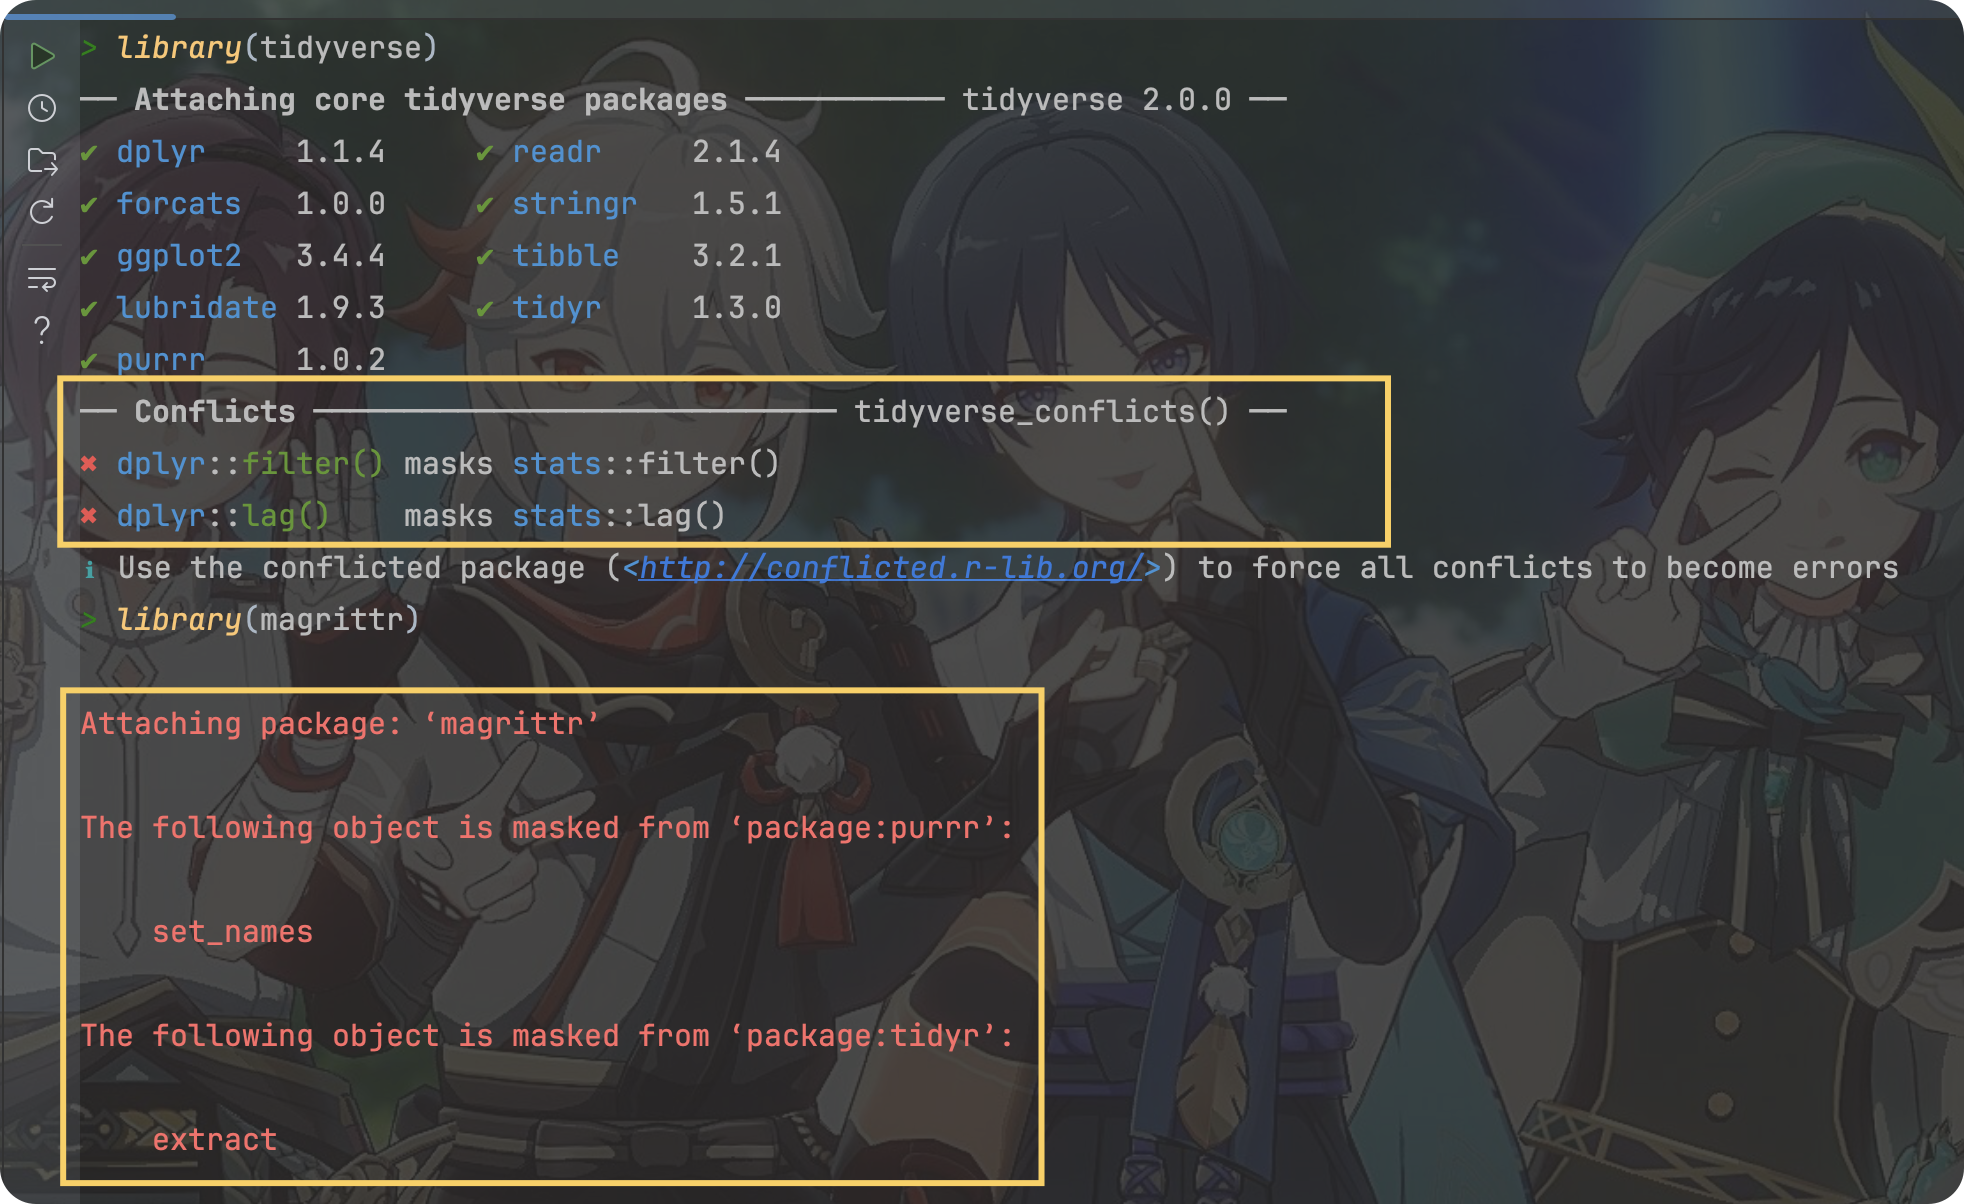
\includegraphics{/Users/lucas/Library/Mobile Documents/com~apple~CloudDocs/~~aa Study Materials/Grade 2 I/Learning/R for Data Science/Review of R/markdown/image/image-20231209213659145.png}

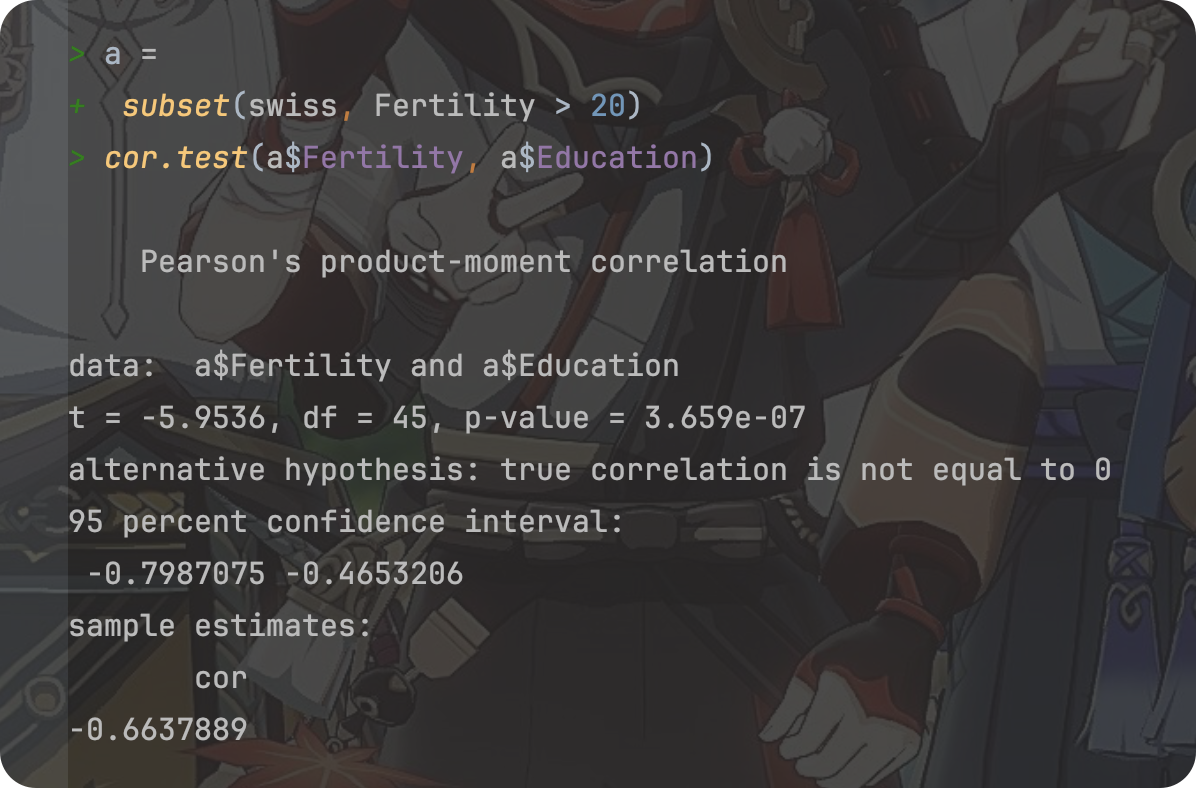
\includegraphics{/Users/lucas/Library/Mobile Documents/com~apple~CloudDocs/~~aa Study Materials/Grade 2 I/Learning/R for Data Science/Review of R/markdown/image/image-20231209213728898.png}

The code above can be replaced by:

\begin{Shaded}
\begin{Highlighting}[]
\NormalTok{swiss }\SpecialCharTok{\%\textgreater{}\%}
  \FunctionTok{subset}\NormalTok{(., Fertility }\SpecialCharTok{\textgreater{}} \DecValTok{20}\NormalTok{) }\SpecialCharTok{\%\$\%}
  \FunctionTok{cor.test}\NormalTok{(Education, Fertility)}
\end{Highlighting}
\end{Shaded}

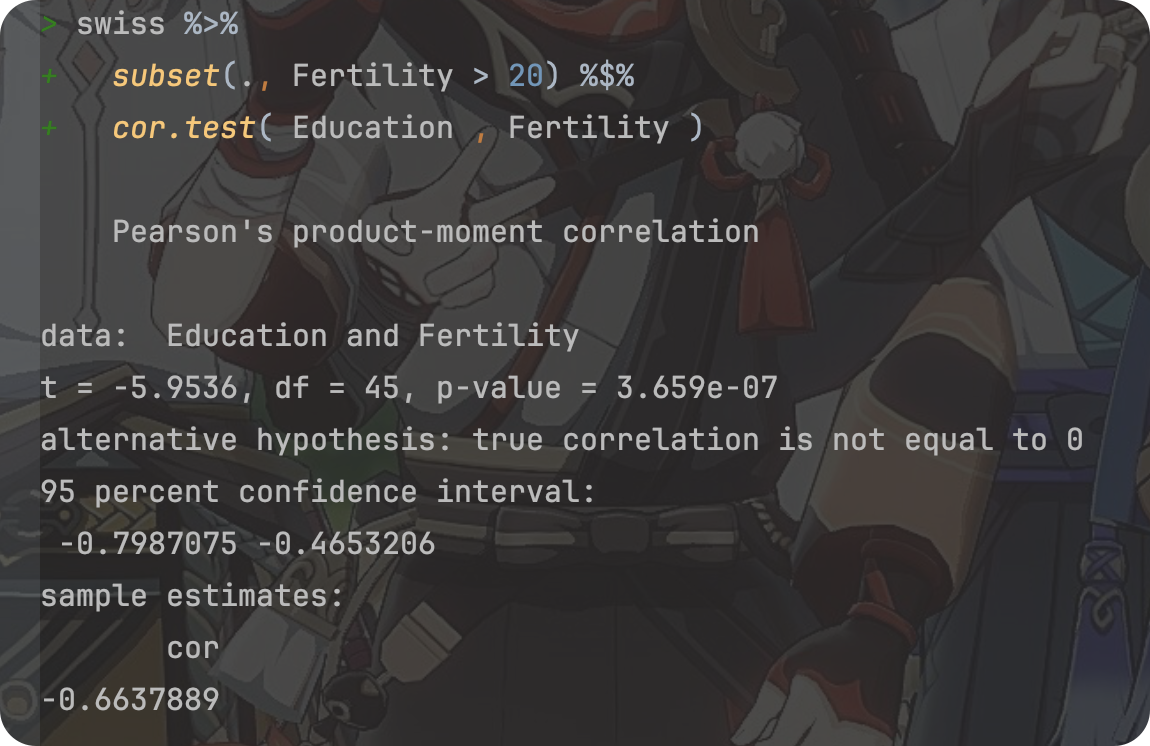
\includegraphics{/Users/lucas/Library/Mobile Documents/com~apple~CloudDocs/~~aa Study Materials/Grade 2 I/Learning/R for Data Science/Review of R/markdown/image/image-20231209214149857.png}

所有函数都支持 pipe,通常需要用 \texttt{.}
指代传递来的数据,并以参数的形式赋予下游函数

\begin{itemize}
\item
  \textbf{\texttt{\%\textgreater{}\%}}:最常见的管道操作符,用于将左侧表达式的结果作为右侧表达式的第一个参数。在这种情况下,右侧表达式的结果会成为整个管道表达式的结果。
\item
  \textbf{\texttt{\%T\textgreater{}\%}
  }:将左侧表达式的结果传递给右侧表达式。然而,与
  \texttt{\%\textgreater{}\%}
  不同的是,整个管道表达式的结果是左侧表达式的结果,而不是右侧表达式的结果。
\item
  \textbf{\texttt{\%\$\%}
  }:允许你在管道的右侧直接访问左侧对象的内部元素,而无需重复指定左侧对象的名称。特别适合用于那些需要从同一个数据对象中提取多个元素进行操作的情况,这在处理复杂的表达式时特别有用,可以使代码更加简洁和清晰。
\item
  \textbf{\texttt{\%\textless{}\textgreater{}\%} }:结合了
  \texttt{\%\textgreater{}\%}
  和赋值操作的功能,允许你在对一个对象进行操作的同时更新这个对象本身。这意味着你可以在管道中对一个对象进行一系列的操作,并且这些操作的结果会直接反映到原始对象上,而不需要进行额外的赋值步骤。特别适用于数据处理和清理的场景,其中你需要对一个数据对象进行一系列的操作,并希望操作的结果直接更新到这个对象上。这样可以使得代码更加整洁,并减少潜在的错误,因为你不需要记住为每个中间步骤创建一个新的变量。
\end{itemize}

\hypertarget{egs}{%
\subsubsection{egs:}\label{egs}}

\begin{itemize}
\item
  \texttt{\%T\textgreater{}\%}: 返回上游值 (left-side
  values),操作符在那些需要执行某些操作但不改变原始数据的场景中非常有用。例如,你可能想要打印或绘制原始数据的某些特性,同时保持数据本身不变以便后续操作。
\end{itemize}

\begin{Shaded}
\begin{Highlighting}[]
\NormalTok{res1 }\OtherTok{\textless{}{-}} 
  \FunctionTok{rnorm}\NormalTok{(}\DecValTok{100}\NormalTok{) }\SpecialCharTok{\%\textgreater{}\%}
    \FunctionTok{matrix}\NormalTok{(}\AttributeTok{ncol =} \DecValTok{2}\NormalTok{) }\SpecialCharTok{\%\textgreater{}\%}
    \FunctionTok{plot}\NormalTok{()}\CommentTok{\#此步骤将整个流程的结果赋值给 res1。但 plot() 函数不会返回数据,所以 res1 将不包含任何数据。}

\NormalTok{res2 }\OtherTok{\textless{}{-}} 
  \FunctionTok{rnorm}\NormalTok{(}\DecValTok{100}\NormalTok{) }\SpecialCharTok{\%\textgreater{}\%}
    \FunctionTok{matrix}\NormalTok{(}\AttributeTok{ncol =} \DecValTok{2}\NormalTok{) }\SpecialCharTok{\%T\textgreater{}\%}
    \FunctionTok{plot}\NormalTok{();}\CommentTok{\#由于使用 \%T\textgreater{}\%,res2 将包含步骤 2 中生成的矩阵,而不是 plot() 的输出}
\end{Highlighting}
\end{Shaded}

\begin{itemize}
\item
  \texttt{\%\$\textgreater{}\%}: Attach \ldots{}
\end{itemize}

\begin{Shaded}
\begin{Highlighting}[]
\FunctionTok{attach}\NormalTok{( mtcars ); }\DocumentationTok{\#\# note the warning message ... }
\FunctionTok{cor.test}\NormalTok{( cyl, mpg ); }\DocumentationTok{\#\# 汽缸数与燃油效率}

\FunctionTok{detach}\NormalTok{( mtcars );}
\FunctionTok{with}\NormalTok{( mtcars, }\FunctionTok{cor.test}\NormalTok{( cyl, mpg ) );}

\NormalTok{mtcars }\SpecialCharTok{\%\$\%} 
\FunctionTok{cor.test}\NormalTok{( cyl, mpg );}
\end{Highlighting}
\end{Shaded}

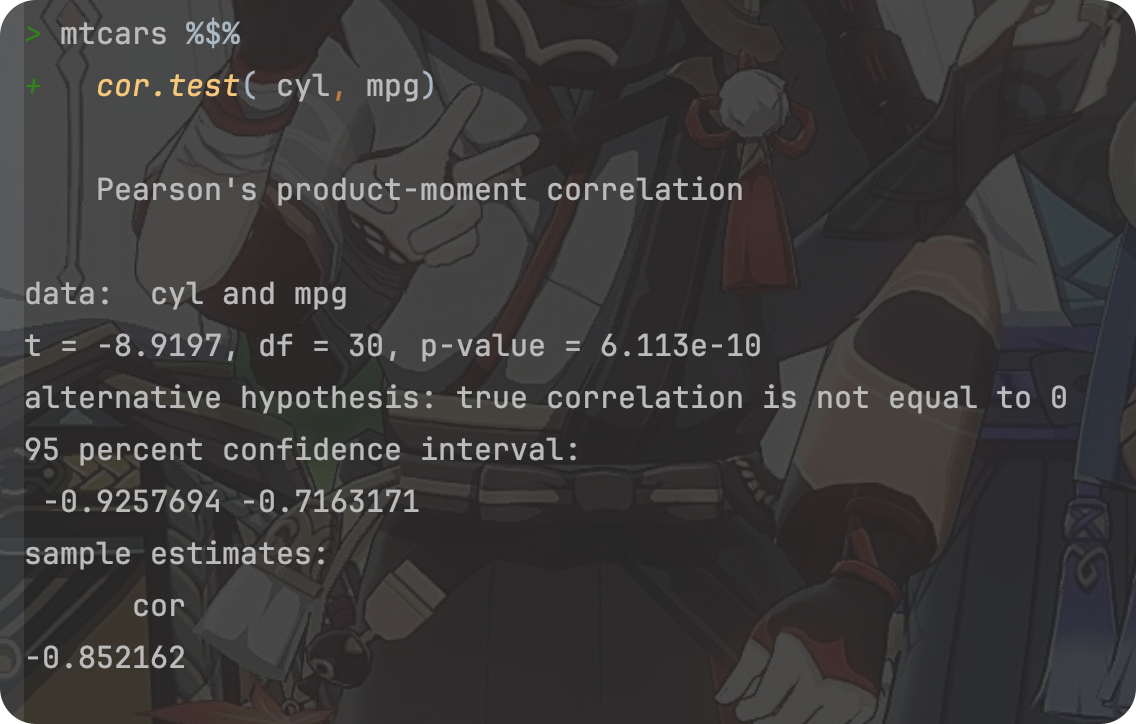
\includegraphics{/Users/lucas/Library/Mobile Documents/com~apple~CloudDocs/~~aa Study Materials/Grade 2 I/Learning/R for Data Science/Review of R/markdown/image/image-20231209220347602.png}

\begin{itemize}
\item
  \texttt{\%\textless{}\textgreater{}\%}
\end{itemize}

\begin{Shaded}
\begin{Highlighting}[]
\DocumentationTok{\#\# 双向 pipe }
\NormalTok{mtcars }\SpecialCharTok{\%\textless{}\textgreater{}\%} \FunctionTok{transform}\NormalTok{(}\AttributeTok{cyl =}\NormalTok{ cyl }\SpecialCharTok{*} \DecValTok{2}\NormalTok{);}
\end{Highlighting}
\end{Shaded}

\hypertarget{attention}{%
\paragraph{\texorpdfstring{\textbf{ATTENTION}}{ATTENTION}}\label{attention}}

\begin{enumerate}
\def\labelenumi{\arabic{enumi}.}
\item
  pipe 的使用可以使思路更清晰
\end{enumerate}

\begin{itemize}
\item
  因此,尽量使用 \texttt{\%\textgreater{}\%}
  (方向明确),而不使用其它方向不明确的 pipe
\end{itemize}

\begin{center}\rule{0.5\linewidth}{0.5pt}\end{center}

\hypertarget{data-wrangler---dplyr}{%
\subsection{\texorpdfstring{Data Wrangler -
\texttt{dplyr}}{Data Wrangler - dplyr}}\label{data-wrangler---dplyr}}

\hypertarget{what-is-dplyr}{%
\subsubsection{\texorpdfstring{What is
\texttt{dplyr}?}{What is dplyr?}}\label{what-is-dplyr}}

\begin{itemize}
\item
  The next iteration of \texttt{plyr},
\item
  Focusing on only data frames (also tibble),
\item
  Row-based manipulation,
\item
  \texttt{dplyr} is faster and has a more consistent API.
\end{itemize}

\texttt{dplyr} provides a consistent set of verbs that help you
\textbf{solve the most common data manipulation challenges}:

\begin{enumerate}
\def\labelenumi{\arabic{enumi}.}
\item
  \texttt{select()}
\end{enumerate}

\begin{itemize}
\item
  \textbf{功能}:\texttt{select()} 用于从数据框中选择一列或多列。
\item
  \textbf{常见用法}:\texttt{select(data,\ column1,\ column2,\ ...)}
\item
  参数

  \begin{itemize}
  \item
    \texttt{data}:数据框对象。
  \item
    \texttt{column1,\ column2,\ ...}:要选择的列的名称。
  \end{itemize}
\end{itemize}

\begin{enumerate}
\def\labelenumi{\arabic{enumi}.}
\item
  \texttt{filter()}
\end{enumerate}

\begin{itemize}
\item
  \textbf{功能}:\texttt{filter()} 用于根据条件筛选数据框中的行。
\item
  \textbf{常见用法}:\texttt{filter(data,\ condition)}
\item
  参数

  \begin{itemize}
  \item
    \texttt{data}:数据框对象。
  \item
    \texttt{condition}:筛选条件,可以是逻辑表达式。
  \end{itemize}
\end{itemize}

\begin{enumerate}
\def\labelenumi{\arabic{enumi}.}
\item
  \texttt{mutate()}
\end{enumerate}

\begin{itemize}
\item
  \textbf{功能}:\texttt{mutate()} 用于在数据框中添加新列或修改现有列。
\item
  \textbf{常见用法}:\texttt{mutate(data,\ new\_column\ =\ expression)}
\item
  参数

  \begin{itemize}
  \item
    \texttt{data}:数据框对象。
  \item
    \texttt{new\_column\ =\ expression}:创建或修改列的表达式。
  \end{itemize}
\end{itemize}

\begin{enumerate}
\def\labelenumi{\arabic{enumi}.}
\item
  \texttt{summarise()}
\end{enumerate}

\begin{itemize}
\item
  \textbf{功能}:\texttt{summarise()}
  用于对数据框中的数据进行汇总或聚合操作。
\item
  \textbf{常见用法}:\texttt{summarise(data,\ summary\ =\ function(column))}
\item
  参数

  \begin{itemize}
  \item
    \texttt{data}:数据框对象。
  \item
    \texttt{summary\ =\ function(column)}:汇总或聚合操作,如求和、平均等。
  \end{itemize}
\end{itemize}

\begin{enumerate}
\def\labelenumi{\arabic{enumi}.}
\item
  \texttt{arrange()}
\end{enumerate}

\begin{itemize}
\item
  \textbf{功能}:\texttt{arrange()}
  用于根据一列或多列对数据框中的行进行排序。
\item
  \textbf{常见用法}:\texttt{arrange(data,\ column)}
\item
  参数

  \begin{itemize}
  \item
    \texttt{data}:数据框对象。
  \item
    \texttt{column}:用于排序的列。可以添加多列进行多级排序。
  \end{itemize}
\end{itemize}

\hypertarget{eg}{%
\subsection{e.g.}\label{eg}}

\hypertarget{ux67e5ux770b-mousetibble-ux7684ux5185ux5bb9}{%
\subsubsection{查看 mouse.tibble
的内容}\label{ux67e5ux770b-mousetibble-ux7684ux5185ux5bb9}}

\begin{Shaded}
\begin{Highlighting}[]
\CommentTok{\# Read the file}
\FunctionTok{library}\NormalTok{(tidyverse)}
\NormalTok{mouse.tibble }\OtherTok{=}
  \FunctionTok{read\_delim}\NormalTok{(}
    \AttributeTok{file =} \StringTok{"data/mouse\_genes\_biomart\_sep2018.txt"}\NormalTok{,}
    \AttributeTok{delim =} \StringTok{"}\SpecialCharTok{\textbackslash{}t}\StringTok{"}\NormalTok{,}
    \AttributeTok{quote =} \StringTok{""}\NormalTok{,}
    \AttributeTok{show\_col\_types =} \ConstantTok{FALSE}
\NormalTok{  )}

\CommentTok{\# View mouse.tibble content}
\NormalTok{ttype.stats }\OtherTok{=}
\NormalTok{  mouse.tibble }\SpecialCharTok{\%\textgreater{}\%}
    \FunctionTok{count}\NormalTok{(}\StringTok{\textasciigrave{}}\AttributeTok{Transcript type}\StringTok{\textasciigrave{}}\NormalTok{) }\SpecialCharTok{\%\textgreater{}\%}
    \FunctionTok{arrange}\NormalTok{(}\SpecialCharTok{{-}}\NormalTok{n)}

\CommentTok{\# View mouse.tibble content, cont.}
\NormalTok{chr.stats }\OtherTok{=}
\NormalTok{  mouse.tibble }\SpecialCharTok{\%\textgreater{}\%}
    \FunctionTok{count}\NormalTok{(}\StringTok{\textasciigrave{}}\AttributeTok{Chromosome/scaffold name}\StringTok{\textasciigrave{}}\NormalTok{) }\SpecialCharTok{\%\textgreater{}\%}
    \FunctionTok{arrange}\NormalTok{(}\SpecialCharTok{{-}}\NormalTok{n)}
\end{Highlighting}
\end{Shaded}

\hypertarget{ux5206ux6790ux4efbux52a1}{%
\subsubsection{分析任务}\label{ux5206ux6790ux4efbux52a1}}

\begin{enumerate}
\def\labelenumi{\arabic{enumi}.}
\item
  将染色体限制在常染色体和XY上(去掉未组装的小片段) ; 处理行
\item
  将基因类型限制在 protein\_coding, miRNA和 lincRNA 这三种;处理行
\item
  统计每条染色体上不同类型基因(protein\_coding, miRNA, lincRNA)的数量
\item
  按染色体(正)、基因数量(倒)进行排序
\end{enumerate}

\hypertarget{ux7528-dplyr-ux5b9eux73b0}{%
\subsubsection{\texorpdfstring{用 \texttt{dplyr}
实现}{用 dplyr 实现}}\label{ux7528-dplyr-ux5b9eux73b0}}

\begin{Shaded}
\begin{Highlighting}[]
\NormalTok{dat }\OtherTok{\textless{}{-}}\NormalTok{ mouse.tibble }\SpecialCharTok{\%\textgreater{}\%} 
  \DocumentationTok{\#\# 1. }
  
  \FunctionTok{filter}\NormalTok{( }\StringTok{\textasciigrave{}}\AttributeTok{Chromosome/scaffold name}\StringTok{\textasciigrave{}} \SpecialCharTok{\%in\%} \FunctionTok{c}\NormalTok{( }\DecValTok{1}\SpecialCharTok{:}\DecValTok{19}\NormalTok{, }\StringTok{"X"}\NormalTok{, }\StringTok{"Y"}\NormalTok{ )   ) }\SpecialCharTok{\%\textgreater{}\%} 
  
  \DocumentationTok{\#\# 2. }
  \FunctionTok{filter}\NormalTok{( }\StringTok{\textasciigrave{}}\AttributeTok{Transcript type}\StringTok{\textasciigrave{}} \SpecialCharTok{\%in\%} \FunctionTok{c}\NormalTok{( }\StringTok{"protein\_coding"}\NormalTok{, }\StringTok{"miRNA"}\NormalTok{, }\StringTok{"lincRNA"}\NormalTok{ ) ) }\SpecialCharTok{\%\textgreater{}\%}
  
  \DocumentationTok{\#\# change column name ... }
  \FunctionTok{select}\NormalTok{( }\AttributeTok{CHR =} \StringTok{\textasciigrave{}}\AttributeTok{Chromosome/scaffold name}\StringTok{\textasciigrave{}}\NormalTok{, }\AttributeTok{TYPE =} \StringTok{\textasciigrave{}}\AttributeTok{Transcript type}\StringTok{\textasciigrave{}}\NormalTok{, }
          \AttributeTok{GENE\_ID =} \StringTok{\textasciigrave{}}\AttributeTok{Gene stable ID}\StringTok{\textasciigrave{}}\NormalTok{, }
          \AttributeTok{GENE\_LEN =}  \StringTok{\textasciigrave{}}\AttributeTok{Transcript length (including UTRs and CDS)}\StringTok{\textasciigrave{}}\NormalTok{  ) }\SpecialCharTok{\%\textgreater{}\%}
  
  \DocumentationTok{\#\# 3. }
  \FunctionTok{group\_by}\NormalTok{( CHR, TYPE ) }\SpecialCharTok{\%\textgreater{}\%} 
  \FunctionTok{summarise}\NormalTok{( }\AttributeTok{count =} \FunctionTok{n\_distinct}\NormalTok{( GENE\_ID ), }\AttributeTok{mean\_len =} \FunctionTok{mean}\NormalTok{( GENE\_LEN ) ) }\SpecialCharTok{\%\textgreater{}\%} 
  
  \DocumentationTok{\#\# 4. }
  \FunctionTok{arrange}\NormalTok{(  CHR  , }\FunctionTok{desc}\NormalTok{( count ) );}
\end{Highlighting}
\end{Shaded}

\hypertarget{ux68c0ux67e5ux8fd0ux884cux7ed3ux679c}{%
\subsubsection{检查运行结果}\label{ux68c0ux67e5ux8fd0ux884cux7ed3ux679c}}

\begin{Shaded}
\begin{Highlighting}[]
\NormalTok{knitr}\SpecialCharTok{::}\FunctionTok{kable}\NormalTok{( }\FunctionTok{head}\NormalTok{( dat, }\AttributeTok{n =} \DecValTok{15}\NormalTok{ ) );}

\NormalTok{CHR	TYPE	          count	mean\_len}
\DecValTok{1}\NormalTok{	  protein\_coding	}\DecValTok{1200}	\FloatTok{2699.59009}
\DecValTok{1}\NormalTok{	  lincRNA	        }\DecValTok{347}	  \FloatTok{1206.76149}
\DecValTok{1}\NormalTok{	  miRNA	          }\DecValTok{128}	  \FloatTok{97.97656}
\DecValTok{10}\NormalTok{	protein\_coding	}\DecValTok{1020}	\FloatTok{2408.16454}
\DecValTok{10}\NormalTok{	lincRNA	        }\DecValTok{398}  	\FloatTok{1220.35543}
\DecValTok{10}\NormalTok{	miRNA	          }\DecValTok{91}	  \FloatTok{89.87912}
\DecValTok{11}\NormalTok{	protein\_coding	}\DecValTok{1640}	\FloatTok{2431.87666}
\DecValTok{11}\NormalTok{	lincRNA	        }\DecValTok{189} 	\FloatTok{1134.49174}
\DecValTok{11}\NormalTok{	miRNA	          }\DecValTok{137}	  \FloatTok{87.48905}
\DecValTok{12}\NormalTok{	protein\_coding	}\DecValTok{644}	  \FloatTok{2523.94822}
\DecValTok{12}\NormalTok{	lincRNA	        }\DecValTok{327}	  \FloatTok{1277.14979}
\DecValTok{12}\NormalTok{	miRNA	          }\DecValTok{146}	  \FloatTok{86.24658}
\DecValTok{13}\NormalTok{	protein\_coding	}\DecValTok{831}	  \FloatTok{2380.41499}
\DecValTok{13}\NormalTok{	lincRNA	        }\DecValTok{428}	  \FloatTok{1251.04552}
\DecValTok{13}\NormalTok{	miRNA	          }\DecValTok{97}	  \FloatTok{105.52577}
\end{Highlighting}
\end{Shaded}

\begin{center}\rule{0.5\linewidth}{0.5pt}\end{center}

\newpage
\hypertarget{r-for-bioinformatics-data-wrangler-part-2}{%
\section{R for bioinformatics, data wrangler, part
2}\label{r-for-bioinformatics-data-wrangler-part-2}}

\begin{quote}
Talk 06
\end{quote}

\hypertarget{tidyr}{%
\subsection{\texorpdfstring{\texttt{tidyr}}{tidyr}}\label{tidyr}}

\begin{itemize}
\item
  \texttt{pivot\_longer()} to take the place of \texttt{gather}
\item
  \texttt{pivot\_wider()} to take the place of \texttt{spread}
\end{itemize}

\hypertarget{data-wrangler---tidyr}{%
\subsection{\texorpdfstring{Data Wrangler -
\texttt{tidyr}}{Data Wrangler - tidyr}}\label{data-wrangler---tidyr}}

You can get \texttt{tidyr} in the package set \texttt{tidyverse}, or
simply install it the first time you want to use it via
\texttt{install.packages("tidyr")}.

\hypertarget{ux5bbdux6570ux636eux7684ux7279ux70b9}{%
\subsection{宽数据的特点}\label{ux5bbdux6570ux636eux7684ux7279ux70b9}}

\hypertarget{ux4f18ux70b9}{%
\subsubsection{优点:}\label{ux4f18ux70b9}}

\begin{itemize}
\item
  自然,易理解;
\end{itemize}

\hypertarget{ux7f3aux70b9}{%
\subsubsection{缺点:}\label{ux7f3aux70b9}}

\begin{itemize}
\item
  不易处理;
\item
  稀疏时问题较大;
\end{itemize}

\hypertarget{the-usage-of-tidyr}{%
\subsubsection{\texorpdfstring{The usage of
\texttt{tidyr}}{The usage of tidyr}}\label{the-usage-of-tidyr}}

\begin{itemize}
\item
  宽和长数据的相互转换
\end{itemize}

\begin{Shaded}
\begin{Highlighting}[]
\CommentTok{\# Eg 1}
\FunctionTok{library}\NormalTok{(tidyverse)}
\NormalTok{grades2 }\OtherTok{=}
	\FunctionTok{read\_tsv}\NormalTok{(}\AttributeTok{file =} \StringTok{"data/grades2.txt"}\NormalTok{)}

\NormalTok{grades3 }\OtherTok{=}
\NormalTok{	grades2 }\SpecialCharTok{\%\textgreater{}\%} 
	\FunctionTok{pivot\_longer}\NormalTok{( }
    \SpecialCharTok{{-}}\NormalTok{ name,}\CommentTok{\#所有除 name 列之外的列将被转换为长格式。}
    \AttributeTok{names\_to =} \StringTok{"course"}\NormalTok{,}\CommentTok{\#宽格式中的列名(如课程名称)将被转换并存储在名为 course 的新列中。}
    \AttributeTok{values\_to =} \StringTok{"grade"}\CommentTok{\#原始数据框中的值(如成绩)将被转换并存储在名为 grade 的新列中。}
\NormalTok{  )}

\CommentTok{\# Eg 2}
\NormalTok{grades3\_wide }\OtherTok{=}\NormalTok{ grades3\_long }\SpecialCharTok{\%\textgreater{}\%} 
  \FunctionTok{pivot\_wider}\NormalTok{(}
    \AttributeTok{names\_from =} \StringTok{"course"}\NormalTok{,}\CommentTok{\# course 列的值将成为宽格式数据框的新列名。}
    \AttributeTok{values\_from =} \StringTok{"grade"}\CommentTok{\#grade 列的值将填充到相应的新列中。}
\NormalTok{  )}
\end{Highlighting}
\end{Shaded}

\hypertarget{if-you-meet-na-in-the-1st-example-you-can-do-like-this}{%
\subsubsection{\texorpdfstring{If you meet \texttt{NA} in the 1st
example, you can do like
this:}{If you meet NA in the 1st example, you can do like this:}}\label{if-you-meet-na-in-the-1st-example-you-can-do-like-this}}

\begin{Shaded}
\begin{Highlighting}[]
\NormalTok{grades3\_1 }\OtherTok{=}
\NormalTok{	grades3[}\SpecialCharTok{!}\FunctionTok{is.na}\NormalTok{(grades3}\SpecialCharTok{\$}\NormalTok{grade), ]}
\NormalTok{grades3\_2 }\OtherTok{=}
\NormalTok{	grades3[}\FunctionTok{complete.cases}\NormalTok{(grades3), ]}

\CommentTok{\# A better solution}
\NormalTok{grades3\_long }\OtherTok{=}\NormalTok{ grades2 }\SpecialCharTok{\%\textgreater{}\%} 
  \FunctionTok{pivot\_longer}\NormalTok{( }\SpecialCharTok{{-}}\NormalTok{ name, }
                \AttributeTok{names\_to =} \StringTok{"course"}\NormalTok{, }
                \AttributeTok{values\_to =} \StringTok{"grade"}\NormalTok{,}
                 \AttributeTok{values\_drop\_na =}\NormalTok{ TRUE}\CommentTok{\#删除任何包含 NA 的行。结果中只会包含完整的、没有缺失值的记录。}
\NormalTok{              )}

\CommentTok{\# Pay attention to the variant named "values\_drop\_na"}
\end{Highlighting}
\end{Shaded}

\hypertarget{more-functions-in-tidyr-see--httpsr4dshadleynzdata-tidyhtml}{%
\subsubsection{\texorpdfstring{More functions in \texttt{tidyr}: (See @
\url{https://r4ds.hadley.nz/data-tidy.html})}{More functions in tidyr: (See @ https://r4ds.hadley.nz/data-tidy.html)}}\label{more-functions-in-tidyr-see--httpsr4dshadleynzdata-tidyhtml}}

\hypertarget{tidyrseparate}{%
\subsubsection{\texorpdfstring{\texttt{tidyr::separate()}}{tidyr::separate()}}\label{tidyrseparate}}

将包含多个信息的单一列分割成多个列,以便于进行更深入的数据分析和可视化。

\begin{itemize}
\item
  \texttt{data}: 数据框。
\item
  \texttt{col}: 需要被分割的列。
\item
  \texttt{into}: 一个字符串向量,包含新列的名称。
\item
  \texttt{sep}: 分割符号。默认是非字母数字字符。
\item
  \texttt{remove}: 是否移除原始列,默认为 \texttt{TRUE}。
\item
  \texttt{convert}: 如果设置为
  \texttt{TRUE},尝试自动将分割后的字符串转换为适当的数据类型。
\end{itemize}

\textbf{Usage:}

\begin{Shaded}
\begin{Highlighting}[]
\FunctionTok{separate}\NormalTok{(}
\NormalTok{  data,}
\NormalTok{  col,}
\NormalTok{  into,}
  \AttributeTok{sep =} \StringTok{"[\^{}[:alnum:]]+"}\NormalTok{,}
  \AttributeTok{remove =} \ConstantTok{TRUE}\NormalTok{,}
  \AttributeTok{convert =} \ConstantTok{FALSE}\NormalTok{,}
  \AttributeTok{extra =} \StringTok{"warn"}\NormalTok{,}
  \AttributeTok{fill =} \StringTok{"warn"}\NormalTok{,}
\NormalTok{  ...}
\NormalTok{)}

\CommentTok{\# Default parameters are listed.}
\end{Highlighting}
\end{Shaded}

\hypertarget{tidyrunite}{%
\subsubsection{\texorpdfstring{\texttt{tidyr::unite()}}{tidyr::unite()}}\label{tidyrunite}}

将多个列合并成一个单独的列。

\begin{itemize}
\item
  \texttt{data}: 数据框。
\item
  \texttt{new\_col}: 合并后的新列的名称。
\item
  \texttt{col1,\ col2,\ ...}: 需要合并的列。
\item
  \texttt{sep}: 合并时使用的分隔符,默认为下划线(\texttt{\_})。
\item
  \texttt{remove}: 是否移除原始列,默认为 \texttt{TRUE}。
\end{itemize}

\textbf{Usage:}

\begin{Shaded}
\begin{Highlighting}[]
\FunctionTok{unite}\NormalTok{(}
\NormalTok{  data,}
\NormalTok{  new\_col, }
\NormalTok{  col1, col2, ..., }
  \AttributeTok{sep =} \StringTok{"\_"}\NormalTok{, }
  \AttributeTok{remove =} \ConstantTok{TRUE}\NormalTok{, }
  \AttributeTok{na.rm =} \ConstantTok{FALSE}
\NormalTok{)}

\CommentTok{\# Default parameters are listed.}
\end{Highlighting}
\end{Shaded}

\begin{center}\rule{0.5\linewidth}{0.5pt}\end{center}

\newpage
\hypertarget{r-for-bioinformatics-strings-and-regular-expression}{%
\section{R for bioinformatics, Strings and regular
expression}\label{r-for-bioinformatics-strings-and-regular-expression}}

\begin{quote}
Talk 07
\end{quote}

\hypertarget{stringr}{%
\subsection{\texorpdfstring{\texttt{stringr}}{stringr}}\label{stringr}}

\begin{enumerate}
\def\labelenumi{\arabic{enumi}.}
\item
  basics
\end{enumerate}

\begin{itemize}
\item
  length
\item
  uppercase, lowercase
\item
  unite, separate
\item
  string comparisons, sub string
\end{itemize}

\begin{enumerate}
\def\labelenumi{\arabic{enumi}.}
\item
  regular expression
\end{enumerate}

Before you start\ldots{}

\begin{Shaded}
\begin{Highlighting}[]
\FunctionTok{library}\NormalTok{(stringr)}
\end{Highlighting}
\end{Shaded}

\hypertarget{also-notice-other-famous-packages-used-to-manipulating-string}{%
\subsubsection{Also notice other famous packages used to manipulating
string:}\label{also-notice-other-famous-packages-used-to-manipulating-string}}

\texttt{stringi}(Following are based on the official R Documentation)

\hypertarget{description}{%
\paragraph{\texorpdfstring{\textbf{Description}}{Description}}\label{description}}

\texttt{stringi} is THE R package for fast, correct, consistent, and
convenient string/text manipulation. It gives predictable results on
every platform, in each locale, and under any native character encoding.

\begin{center}\rule{0.5\linewidth}{0.5pt}\end{center}

\hypertarget{usage-of-writelines-from-official-r-documentation}{%
\subsubsection{\texorpdfstring{Usage of \texttt{writeLines()} (from
official R
Documentation)}{Usage of writeLines() (from official R Documentation)}}\label{usage-of-writelines-from-official-r-documentation}}

\hypertarget{description-2}{%
\paragraph{Description}\label{description-2}}

Write text lines to a connection.

\hypertarget{usage}{%
\paragraph{Usage}\label{usage}}

\begin{Shaded}
\begin{Highlighting}[]
\NormalTok{writeLines(text, con = stdout(), sep = "\textbackslash{}n", useBytes = FALSE)}
\end{Highlighting}
\end{Shaded}

\hypertarget{arguments}{%
\paragraph{Arguments}\label{arguments}}

\begin{longtable}[]{@{}ll@{}}
\toprule\noalign{}
\texttt{text} & A character vector \\
\midrule\noalign{}
\endhead
\bottomrule\noalign{}
\endlastfoot
\texttt{con} & A
\href{vscode-webview://00i87qrgljff0t3jmc9gjufilst9usetvkh9gn773om0ic67o1j2/base/help/connection}{connection}
object or a character string. \\
\texttt{sep} & character string. A string to be written to the
connection after each line of text. \\
\texttt{useBytes} & logical. See `Details'. \\
\end{longtable}

\hypertarget{details}{%
\paragraph{Details}\label{details}}

如果\texttt{con}是一个字符串,函数调用\texttt{file}来获得一个文件连接,该文件连接在函数调用期间被打开。
(\href{vscode-webview://00i87qrgljff0t3jmc9gjufilst9usetvkh9gn773om0ic67o1j2/base/help/tilde\%20expansion}{tilde
expansion} of the file path is done by \texttt{file}.)

如果连接是打开的,则从其当前位置写入。如果未打开,则在\texttt{wt}模式下在调用期间打开,然后再次关闭。

正常情况下,\texttt{writeLines}用于文本模式连接,默认分隔符转换为该平台的正常分隔符(Unix/Linux上为LF,Windows上为CRLF)。为了获得更多的控制,打开一个二进制连接,并在\texttt{sep}中指定要写入文件的精确值。为了更好的控制,在二进制连接上使用\texttt{writeChar}。

\texttt{useBytes} is for expert use. Normally (when false) character
strings with marked encodings are converted to the current encoding
before being passed to the connection (which might do further
re-encoding). \texttt{useBytes\ =\ TRUE} suppresses the re-encoding of
marked strings so they are passed byte-by-byte to the connection: this
can be useful when strings have already been re-encoded by e.g.
\texttt{iconv}. (It is invoked automatically for strings with marked
encoding \texttt{"bytes"}.)

\hypertarget{difference-between-double-quote-and-single-quote}{%
\subsubsection{\texorpdfstring{Difference between double
quote(\texttt{“”}) and single
quote(\texttt{‘’})}{Difference between double quote(``\,'') and single quote(`\,')}}\label{difference-between-double-quote-and-single-quote}}

In R and its string manipulation package \texttt{stringr}, there is no
difference between strings defined with double quotes (\texttt{"}) and
single quotes (\texttt{\textquotesingle{}}). Both are used to define
strings and you can use either depending on your preference or the
situation.

例如,如果字符串包含单引号,您应该用双引号将字符串括起来,反之亦然。Here\textquotesingle s
an example:

\begin{Shaded}
\begin{Highlighting}[]
\CommentTok{\# Using double quotes when the string contains a single quote}
\NormalTok{string1 }\OtherTok{=} \StringTok{"It\textquotesingle{}s a beautiful day"}

\CommentTok{\# Using single quotes when the string contains a double quote}
\NormalTok{string2 }\OtherTok{=} \StringTok{\textquotesingle{}He said, "Hello, world!"\textquotesingle{}}
\end{Highlighting}
\end{Shaded}

In both cases, R will interpret the contents between the quotes as a
string.

\hypertarget{some-of-the-functions-in-the-stringi-package-are-similar-in-function-to-those-that-come-with-the-system}{%
\subsubsection{\texorpdfstring{Some of the functions in the
\texttt{stringi} package are similar in function to those that come with
the
system.}{Some of the functions in the stringi package are similar in function to those that come with the system.}}\label{some-of-the-functions-in-the-stringi-package-are-similar-in-function-to-those-that-come-with-the-system}}

Here are some functions in the \texttt{stringi} package that share
similar functionalities with base R\textquotesingle s string functions,
along with examples showcasing their differences:

\begin{enumerate}
\def\labelenumi{\arabic{enumi}.}
\item
  \textbf{\texttt{stri\_length()} vs. \texttt{nchar()}}:

  \begin{itemize}
  \item
    \texttt{stri\_length()} in \texttt{stringi} calculates the number of
    code points in a string, accounting for Unicode characters.
  \item
    \texttt{nchar()} in base R counts the number of characters in a
    string, but it might not handle Unicode characters as accurately as
    \texttt{stri\_length()}.
  \end{itemize}

\begin{Shaded}
\begin{Highlighting}[]
\FunctionTok{library}\NormalTok{(stringi)}

\CommentTok{\# Using stri\_length from stringi}
\NormalTok{string }\OtherTok{=} \StringTok{"café"}
\FunctionTok{stri\_length}\NormalTok{(string)}
\CommentTok{\# Output: 4}

\CommentTok{\# Using nchar from base R}
\FunctionTok{nchar}\NormalTok{(string)}
\CommentTok{\# Output: 4}
\end{Highlighting}
\end{Shaded}

  In this example, both \texttt{stri\_length()} and \texttt{nchar()}
  return the same count for ASCII characters. However, when dealing with
  Unicode characters, \texttt{stri\_length()} can accurately count them
  as individual code points, whereas \texttt{nchar()} might not handle
  them correctly.
\item
  \textbf{\texttt{stri\_split\_*()} vs. \texttt{strsplit()}}:

  \begin{itemize}
  \item
    \texttt{stri\_split\_*()} functions in \texttt{stringi} split a
    string based on various criteria like fixed patterns, regular
    expressions, or character classes.
  \item
    \texttt{strsplit()} in base R performs a similar operation but might
    differ in handling certain edge cases and Unicode characters.
  \end{itemize}

\begin{Shaded}
\begin{Highlighting}[]
\CommentTok{\# Using stri\_split\_* from stringi}
\NormalTok{string }\OtherTok{=} \StringTok{"apple, orange, café"}
\FunctionTok{stri\_split\_fixed}\NormalTok{(string, }\AttributeTok{pattern =} \StringTok{", "}\NormalTok{)}
\CommentTok{\# Output: list("apple", "orange", "café")}

\CommentTok{\# Using strsplit from base R}
\FunctionTok{strsplit}\NormalTok{(string, }\AttributeTok{split =} \StringTok{", "}\NormalTok{)}
\CommentTok{\# Output: list("apple", "orange", "caf", "é")}
\end{Highlighting}
\end{Shaded}

  Here, \texttt{stri\_split\_fixed()} correctly splits the string,
  including the accented character "é," while \texttt{strsplit()} treats
  the accented "é" as two separate characters due to how it handles
  Unicode.
\item
  \textbf{\texttt{stri\_detect()} vs. \texttt{grepl()}}:

  \begin{itemize}
  \item
    \texttt{stri\_detect()} in \texttt{stringi} checks if a pattern
    exists in a string and returns a logical value.
  \item
    \texttt{grepl()} in base R performs a similar task but might differ
    in its handling of Unicode characters and certain pattern matching
    options.
  \end{itemize}

\begin{Shaded}
\begin{Highlighting}[]
\CommentTok{\# Using stri\_detect from stringi}
\NormalTok{string }\OtherTok{=} \StringTok{"This is a café"}
\FunctionTok{stri\_detect}\NormalTok{(string, }\AttributeTok{regex =} \StringTok{"café"}\NormalTok{)}
\CommentTok{\# Output: TRUE}

\CommentTok{\# Using grepl from base R}
\FunctionTok{grepl}\NormalTok{(}\StringTok{"café"}\NormalTok{, string)}
\CommentTok{\# Output: FALSE}
\end{Highlighting}
\end{Shaded}

  In this example, \texttt{stri\_detect()} correctly detects the
  presence of the word "café," while \texttt{grepl()} returns a
  different result due to potential differences in Unicode handling or
  pattern matching options.
\end{enumerate}

The examples highlight how \texttt{stringi} functions like
\texttt{stri\_length()}, \texttt{stri\_split\_*()}, and
\texttt{stri\_detect()} differ from their base R counterparts
(\texttt{nchar()}, \texttt{strsplit()}, and \texttt{grepl()}) by
providing more accurate handling of Unicode characters and often more
versatile string manipulation options.

\hypertarget{some-of-the-functions-in-the-stringr-package-are-similar-in-function-to-those-that-come-with-the-system}{%
\subsubsection{\texorpdfstring{Some of the functions in the
\texttt{stringr} package are similar in function to those that come with
the
system.}{Some of the functions in the stringr package are similar in function to those that come with the system.}}\label{some-of-the-functions-in-the-stringr-package-are-similar-in-function-to-those-that-come-with-the-system}}

Here are examples comparing some functions from the \texttt{stringr}
package with their counterparts from base R:

\hypertarget{string-length}{%
\subsubsection{string length}\label{string-length}}

\begin{enumerate}
\def\labelenumi{\arabic{enumi}.}
\item
  \textbf{\texttt{str\_length()} vs. \texttt{nchar()}:}
\end{enumerate}

\begin{Shaded}
\begin{Highlighting}[]
\FunctionTok{library}\NormalTok{(stringr)}

\CommentTok{\# Using str\_length from stringr}
\NormalTok{string }\OtherTok{=} \FunctionTok{c}\NormalTok{(}\StringTok{"apple"}\NormalTok{, }\ConstantTok{NA}\NormalTok{, }\StringTok{"banana"}\NormalTok{, }\StringTok{""}\NormalTok{)}
\FunctionTok{str\_length}\NormalTok{(string)}
\CommentTok{\# Output: 5   NA   6   0}

\CommentTok{\# Using nchar from base R}
\FunctionTok{nchar}\NormalTok{(string)}
\CommentTok{\# Output: 5  NA   6   0}
\end{Highlighting}
\end{Shaded}

\texttt{str\_length()}和\texttt{nchar()}都计算每个字符串元素中的字符数。然而,\texttt{str\_length()}通过返回\texttt{NA}来更一致地处理缺失值,而\texttt{nchar()}在某些情况下可能会以不同的方式处理\texttt{NA}。

\begin{enumerate}
\def\labelenumi{\arabic{enumi}.}
\item
  \textbf{\texttt{str\_sub()} vs. \texttt{substr()}:}
\end{enumerate}

\begin{Shaded}
\begin{Highlighting}[]
\CommentTok{\# Using str\_sub from stringr}
\NormalTok{string }\OtherTok{=} \FunctionTok{c}\NormalTok{(}\StringTok{"hello"}\NormalTok{, }\StringTok{"world"}\NormalTok{, }\StringTok{"example"}\NormalTok{)}
\FunctionTok{str\_sub}\NormalTok{(string, }\AttributeTok{start =} \DecValTok{2}\NormalTok{, }\AttributeTok{end =} \DecValTok{4}\NormalTok{)}
\CommentTok{\# Output: "ell" "orl" "xam"}

\CommentTok{\# Using substr from base R}
\FunctionTok{substr}\NormalTok{(string, }\AttributeTok{start =} \DecValTok{2}\NormalTok{, }\AttributeTok{stop =} \DecValTok{4}\NormalTok{)}
\CommentTok{\# Output: "ell" "orl" "xam"}
\end{Highlighting}
\end{Shaded}

\texttt{str\_sub()}和\texttt{substr()}都根据指定的开始和结束位置提取子字符串。然而,\texttt{str\_sub()}允许负索引从字符串的末尾开始计数,并且它更一致地处理缺失值。

\begin{enumerate}
\def\labelenumi{\arabic{enumi}.}
\item
  \textbf{\texttt{str\_replace()} vs. \texttt{sub()} or
  \texttt{gsub()}:}
\end{enumerate}

\begin{Shaded}
\begin{Highlighting}[]
\CommentTok{\# Using str\_replace from stringr}
\NormalTok{string }\OtherTok{=} \FunctionTok{c}\NormalTok{(}\StringTok{"apple pie"}\NormalTok{, }\StringTok{"banana bread"}\NormalTok{, }\StringTok{"cherry cake"}\NormalTok{)}
\FunctionTok{str\_replace}\NormalTok{(string, }\AttributeTok{pattern =} \StringTok{"a"}\NormalTok{, }\AttributeTok{replacement =} \StringTok{"X"}\NormalTok{)}
\CommentTok{\# Output: "Xpple pie"    "bXnana bread" "cherry cXke" }

\CommentTok{\# Using sub from base R}
\FunctionTok{sub}\NormalTok{(}\AttributeTok{pattern =} \StringTok{"a"}\NormalTok{, }\AttributeTok{replacement =} \StringTok{"X"}\NormalTok{, }\AttributeTok{x =}\NormalTok{ string)}
\CommentTok{\# Output: "Xpple pie" "bXnana bread" "cherry cXke"}
\end{Highlighting}
\end{Shaded}

\texttt{str\_replace()}和\texttt{sub()}都用于替换字符串的部分内容。然而,\texttt{str\_replace()}有一个更直观的界面,与\texttt{sub()}相比,它能更优雅地处理缺失值。

\begin{enumerate}
\def\labelenumi{\arabic{enumi}.}
\item
  \textbf{\texttt{paste()}vs.\texttt{str\_c()}}
\end{enumerate}

\hypertarget{string-combine}{%
\subsubsection{\texorpdfstring{string combine
}{string combine }}\label{string-combine}}

\begin{Shaded}
\begin{Highlighting}[]
\DocumentationTok{\#\# 系统自带}
\FunctionTok{paste}\NormalTok{( }\StringTok{"a"}\NormalTok{, }\StringTok{"b"}\NormalTok{, }\StringTok{"c"}\NormalTok{, }\AttributeTok{sep =} \StringTok{""}\NormalTok{ );}
\CommentTok{\#[1] "abc"}

\DocumentationTok{\#\# stringr }
\FunctionTok{str\_c}\NormalTok{( }\StringTok{"a"}\NormalTok{, }\StringTok{"b"}\NormalTok{, }\StringTok{"c"}\NormalTok{ );}
\CommentTok{\#[1] "abc"}
\end{Highlighting}
\end{Shaded}

\hypertarget{string-comparison}{%
\subsubsection{string comparison}\label{string-comparison}}

\textbf{\texttt{strcmp} 函数:}

\begin{itemize}
\item
  \textbf{参数:}

  \begin{itemize}
  \item
    \texttt{str1}:第一个字符串。
  \item
    \texttt{str2}:第二个字符串。
  \end{itemize}
\item
  \textbf{返回值:}

  \begin{itemize}
  \item
    logical, i.e. \texttt{TRUE} if \texttt{s1} and \texttt{s2} have the
    same length as character vectors and all elements are equal as
    character strings, else \texttt{FALSE}.
  \end{itemize}
\end{itemize}

\textbf{\texttt{strcmpi} 函数:}

\begin{itemize}
\item
  \textbf{参数:}

  \begin{itemize}
  \item
    \texttt{str1}:第一个字符串。
  \item
    \texttt{str2}:第二个字符串。
  \end{itemize}
\item
  \textbf{返回值:}

  \begin{itemize}
  \item
    类似于 \texttt{strcmp},但是在不区分大小写的情况下进行比较。
  \end{itemize}
\end{itemize}

\begin{Shaded}
\begin{Highlighting}[]
\DocumentationTok{\#\# direct comparison ; 可用于排序 ...}
\StringTok{"A"} \SpecialCharTok{\textgreater{}} \StringTok{"abc"}\NormalTok{;}
\CommentTok{\#[1] FALSE}

\DocumentationTok{\#\# }
\FunctionTok{library}\NormalTok{(pracma);}
\FunctionTok{strcmp}\NormalTok{( }\StringTok{"chen"}\NormalTok{, }\StringTok{"chenweihua"}\NormalTok{ );}
\FunctionTok{strcmpi}\NormalTok{( }\StringTok{"chen"}\NormalTok{, }\StringTok{"CHEN"}\NormalTok{ );}

\CommentTok{\#}
\CommentTok{\#[1] FALSE}
\CommentTok{\#[1] TRUE}
\end{Highlighting}
\end{Shaded}

These examples demonstrate how \texttt{stringr} functions can be more
consistent and user-friendly in handling various string operations
compared to their base R counterparts.

\hypertarget{in-the-slide-difference-between-toupper-tolower-and-strireverse}{%
\subsubsection{\texorpdfstring{\textbf{(In the slide)} Difference
between \texttt{toupper()}, \texttt{tolower()} and
\texttt{stri\_reverse()}}{(In the slide) Difference between toupper(), tolower() and stri\_reverse()}}\label{in-the-slide-difference-between-toupper-tolower-and-strireverse}}

The functions \texttt{toupper()} and \texttt{tolower()} in base R and
\texttt{stri\_reverse()} in the \texttt{stringi} package perform similar
tasks, but there are some differences in their functionality and usage:

\begin{enumerate}
\def\labelenumi{\arabic{enumi}.}
\item
  \textbf{\texttt{toupper()} and \texttt{tolower()} in Base R:}

  \begin{itemize}
  \item
    \texttt{toupper()} 将字符串中的字符转换为大写。
  \item
    \texttt{tolower()} 将字符串中的字符转换为小写。
  \end{itemize}

\begin{Shaded}
\begin{Highlighting}[]
\CommentTok{\# Using toupper and tolower from base R}
\NormalTok{string }\OtherTok{=} \StringTok{"Hello World!"}

\FunctionTok{toupper}\NormalTok{(string)}
\CommentTok{\# Output: "HELLO WORLD!"}

\FunctionTok{tolower}\NormalTok{(string)}
\CommentTok{\# Output: "hello world!"}
\end{Highlighting}
\end{Shaded}

  These functions are straightforward and work well for ASCII
  characters, converting them to uppercase or lowercase, respectively.
  However, they might not handle Unicode characters or locale-specific
  transformations.
\item
  \textbf{\texttt{stri\_reverse()} in \texttt{stringi}:}

  \begin{itemize}
  \item
    \texttt{stri\_reverse()}
    颠倒字符串中字符的顺序,包括处理多字节字符和Unicode序列。
  \end{itemize}

\begin{Shaded}
\begin{Highlighting}[]
\FunctionTok{library}\NormalTok{(stringi)}

\CommentTok{\# Using stri\_reverse from stringi}
\NormalTok{string }\OtherTok{=} \StringTok{"café"}

\FunctionTok{stri\_reverse}\NormalTok{(string)}
\CommentTok{\# Output: "éfac"}
\end{Highlighting}
\end{Shaded}

  \texttt{stri\_reverse()} reverses the characters in the string
  accurately, even when dealing with Unicode characters or multibyte
  sequences. It ensures correct reversal of characters irrespective of
  their encoding.
\end{enumerate}

The key distinction lies in the handling of character cases and
character sequence reversal. While \texttt{toupper()} and
\texttt{tolower()} focus on case transformations for ASCII characters,
\texttt{stri\_reverse()} in \texttt{stringi} concentrates on accurately
reversing character sequences, making it more suitable for handling
multibyte characters and Unicode strings.

\hypertarget{tricks}{%
\subsubsection{Tricks}\label{tricks}}

\begin{itemize}
\item
  \texttt{stringi} The functions in the package all start with
  \texttt{stri\_}.
\item
  \texttt{strinr} starts with \texttt{str\_}.
\end{itemize}

\hypertarget{regex---regular-expression}{%
\subsection{Regex - Regular
Expression}\label{regex---regular-expression}}

\begin{enumerate}
\def\labelenumi{\arabic{enumi}.}
\item
  Character classes:What characters are (not) matched?

  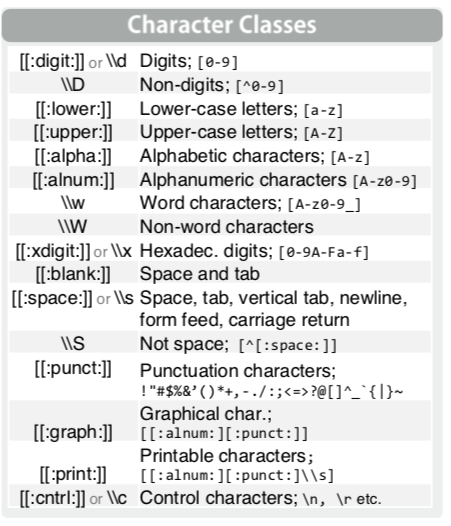
\includegraphics{/Users/lucas/Library/Mobile Documents/com~apple~CloudDocs/~~aa Study Materials/Grade 2 I/Learning/R for Data Science/Review of R/markdown/./image/regular_expression_character_roles.png}
\end{enumerate}

\begin{Shaded}
\begin{Highlighting}[]
\DocumentationTok{\#\# 比如: [ab] 表示寻找a 或 b }
\FunctionTok{c}\NormalTok{( }\StringTok{"abc"}\NormalTok{, }\StringTok{"chen"}\NormalTok{, }\StringTok{"liu"}\NormalTok{, }\StringTok{"blah"}\NormalTok{ ) }\SpecialCharTok{\%\textgreater{}\%} \FunctionTok{str\_subset}\NormalTok{( }\StringTok{"[ab]"}\NormalTok{ );}

\CommentTok{\#[1] "abc"  "blah"}

\DocumentationTok{\#\# 匹配并取出字符中间的数字 }
\FunctionTok{c}\NormalTok{( }\StringTok{"a1334bc"}\NormalTok{, }\StringTok{"ch13e\_45n"}\NormalTok{, }\StringTok{"liu"}\NormalTok{, }\StringTok{"bl00ah"}\NormalTok{ ) }\SpecialCharTok{\%\textgreater{}\%} \FunctionTok{str\_extract}\NormalTok{( }\StringTok{"}\SpecialCharTok{\textbackslash{}\textbackslash{}}\StringTok{d+"}\NormalTok{ );}

\CommentTok{\#[1] "1334" "13"   NA     "00" }
\end{Highlighting}
\end{Shaded}

\begin{Shaded}
\begin{Highlighting}[]
\CommentTok{\# Example 01}
\StringTok{"abc\_123\_??$$\^{}"} \SpecialCharTok{\%\textgreater{}\%} \FunctionTok{str\_extract}\NormalTok{(}\StringTok{"}\SpecialCharTok{\textbackslash{}\textbackslash{}}\StringTok{s+"}\NormalTok{) }\CommentTok{\# Does this string include spaces? }
\StringTok{"abc\_123\_??$$\^{}"} \SpecialCharTok{\%\textgreater{}\%} \FunctionTok{str\_extract}\NormalTok{(}\StringTok{"}\SpecialCharTok{\textbackslash{}\textbackslash{}}\StringTok{d+"}\NormalTok{) }\CommentTok{\# Numbers? }
\StringTok{"abc\_123\_??$$\^{}"} \SpecialCharTok{\%\textgreater{}\%} \FunctionTok{str\_extract}\NormalTok{(}\StringTok{"}\SpecialCharTok{\textbackslash{}\textbackslash{}}\StringTok{w+"}\NormalTok{) }\CommentTok{\# [A{-}z0{-}9\_]}

\NormalTok{[}\DecValTok{1}\NormalTok{] }\ConstantTok{NA}
\NormalTok{[}\DecValTok{1}\NormalTok{] }\StringTok{"123"}
\NormalTok{[}\DecValTok{1}\NormalTok{] }\StringTok{"abc\_123\_"}
\end{Highlighting}
\end{Shaded}

\texttt{str\_extract} : Take out the first match.

\begin{enumerate}
\def\labelenumi{\arabic{enumi}.}
\item
  Matching position

  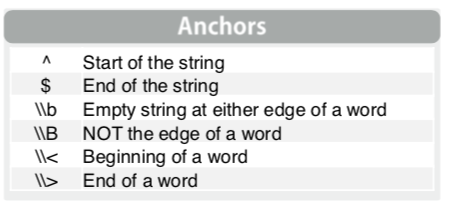
\includegraphics{/Users/lucas/Library/Mobile Documents/com~apple~CloudDocs/~~aa Study Materials/Grade 2 I/Learning/R for Data Science/Review of R/markdown/image/regexpr_anchors.png}
\end{enumerate}

\begin{Shaded}
\begin{Highlighting}[]
\CommentTok{\# Example 02}
\CommentTok{\# STRING ending in \textquotesingle{}wei\textquotesingle{}}
\FunctionTok{c}\NormalTok{(}\StringTok{"chen wei hua"}\NormalTok{, }\StringTok{"chen wei"}\NormalTok{, }\StringTok{"chen"}\NormalTok{) }\SpecialCharTok{\%\textgreater{}\%} \FunctionTok{str\_subset}\NormalTok{(}\StringTok{"wei\$"}\NormalTok{)}

\CommentTok{\#[1] "chen wei"}

\CommentTok{\# CHARACTER ending in \textquotesingle{}wei\textquotesingle{} }
\FunctionTok{c}\NormalTok{(}\StringTok{"chen wei hua"}\NormalTok{, }\StringTok{"chen wei"}\NormalTok{, }\StringTok{"chen"}\NormalTok{) }\SpecialCharTok{\%\textgreater{}\%} \FunctionTok{str\_subset}\NormalTok{(}\StringTok{"wei}\SpecialCharTok{\textbackslash{}\textbackslash{}}\StringTok{b"}\NormalTok{)}

\CommentTok{\#[1] "chen wei hua" "chen wei"   }
\end{Highlighting}
\end{Shaded}

\begin{enumerate}
\def\labelenumi{\arabic{enumi}.}
\item
  Number of matches
\end{enumerate}

\begin{Shaded}
\begin{Highlighting}[]
\CommentTok{\# Example 03}
\StringTok{"1234abc"} \SpecialCharTok{\%\textgreater{}\%} \FunctionTok{str\_extract}\NormalTok{(}\StringTok{"}\SpecialCharTok{\textbackslash{}\textbackslash{}}\StringTok{d+"}\NormalTok{)}
\StringTok{"1234abc"} \SpecialCharTok{\%\textgreater{}\%} \FunctionTok{str\_extract}\NormalTok{(}\StringTok{"}\SpecialCharTok{\textbackslash{}\textbackslash{}}\StringTok{d\{3\}"}\NormalTok{)}
\StringTok{"1234abc"} \SpecialCharTok{\%\textgreater{}\%} \FunctionTok{str\_extract}\NormalTok{(}\StringTok{"}\SpecialCharTok{\textbackslash{}\textbackslash{}}\StringTok{d\{5,6\}"}\NormalTok{)}
\StringTok{"1234abc"} \SpecialCharTok{\%\textgreater{}\%} \FunctionTok{str\_extract}\NormalTok{(}\StringTok{"}\SpecialCharTok{\textbackslash{}\textbackslash{}}\StringTok{d\{2,6\}"}\NormalTok{)}

\NormalTok{[}\DecValTok{1}\NormalTok{] }\StringTok{"1234"}
\NormalTok{[}\DecValTok{1}\NormalTok{] }\StringTok{"123"}
\NormalTok{[}\DecValTok{1}\NormalTok{] }\ConstantTok{NA}
\NormalTok{[}\DecValTok{1}\NormalTok{] }\StringTok{"1234"}
\end{Highlighting}
\end{Shaded}

\begin{enumerate}
\def\labelenumi{\arabic{enumi}.}
\item
  Classes and groups

  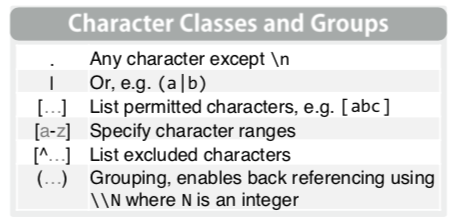
\includegraphics{/Users/lucas/Library/Mobile Documents/com~apple~CloudDocs/~~aa Study Materials/Grade 2 I/Learning/R for Data Science/Review of R/markdown/image/regexprs_classes_groups.png}
\item
  Special characters

  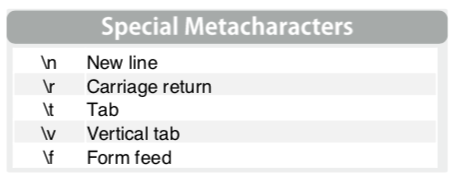
\includegraphics{/Users/lucas/Library/Mobile Documents/com~apple~CloudDocs/~~aa Study Materials/Grade 2 I/Learning/R for Data Science/Review of R/markdown/image/regexprs_special_characters.png}

  \hypertarget{tasks-of-regular-expression}{%
  \subsubsection{\texorpdfstring{tasks of regular expression
  }{tasks of regular expression }}\label{tasks-of-regular-expression}}

  detect patterns : 检查目标string里有无pattern

\begin{Shaded}
\begin{Highlighting}[]
\FunctionTok{grep}\NormalTok{( }\StringTok{"}\SpecialCharTok{\textbackslash{}\textbackslash{}}\StringTok{d+"}\NormalTok{, }\FunctionTok{c}\NormalTok{( }\StringTok{"123"}\NormalTok{, }\StringTok{"abc"}\NormalTok{, }\StringTok{"wei555hua"}\NormalTok{ ) ); }\DocumentationTok{\#\# }
\FunctionTok{grepl}\NormalTok{( }\StringTok{"}\SpecialCharTok{\textbackslash{}\textbackslash{}}\StringTok{d+"}\NormalTok{, }\FunctionTok{c}\NormalTok{( }\StringTok{"123"}\NormalTok{, }\StringTok{"abc"}\NormalTok{, }\StringTok{"wei555hua"}\NormalTok{ ) ); }\DocumentationTok{\#\# }
\FunctionTok{c}\NormalTok{( }\StringTok{"123"}\NormalTok{, }\StringTok{"abc"}\NormalTok{, }\StringTok{"wei555hua"}\NormalTok{ ) }\SpecialCharTok{\%\textgreater{}\%} \FunctionTok{str\_detect}\NormalTok{( }\StringTok{"}\SpecialCharTok{\textbackslash{}\textbackslash{}}\StringTok{d+"}\NormalTok{ );}
\CommentTok{\#}
\NormalTok{[}\DecValTok{1}\NormalTok{] }\DecValTok{1} \DecValTok{3}
\NormalTok{[}\DecValTok{1}\NormalTok{]  }\ConstantTok{TRUE} \ConstantTok{FALSE}  \ConstantTok{TRUE}
\NormalTok{[}\DecValTok{1}\NormalTok{]  }\ConstantTok{TRUE} \ConstantTok{FALSE}  \ConstantTok{TRUE}
\end{Highlighting}
\end{Shaded}

  \textbf{count patterns:统计匹配的数量}

\begin{Shaded}
\begin{Highlighting}[]
\NormalTok{x }\OtherTok{\textless{}{-}} \FunctionTok{c}\NormalTok{(}\StringTok{"why"}\NormalTok{, }\StringTok{"video"}\NormalTok{, }\StringTok{"cross"}\NormalTok{, }\StringTok{"extra"}\NormalTok{, }\StringTok{"deal"}\NormalTok{, }\StringTok{"authority"}\NormalTok{);}
\FunctionTok{str\_detect}\NormalTok{(x, }\StringTok{"[aeiou]"}\NormalTok{);}

\FunctionTok{str\_count}\NormalTok{(x, }\StringTok{"[aeiou]"}\NormalTok{);}
\CommentTok{\#}
\NormalTok{[}\DecValTok{1}\NormalTok{] }\ConstantTok{FALSE}  \ConstantTok{TRUE}  \ConstantTok{TRUE}  \ConstantTok{TRUE}  \ConstantTok{TRUE}  \ConstantTok{TRUE}
\NormalTok{[}\DecValTok{1}\NormalTok{] }\DecValTok{0} \DecValTok{3} \DecValTok{1} \DecValTok{2} \DecValTok{2} \DecValTok{4}
\end{Highlighting}
\end{Shaded}

  locate patterns (定位)

\begin{Shaded}
\begin{Highlighting}[]
\FunctionTok{regexpr}\NormalTok{( }\StringTok{"}\SpecialCharTok{\textbackslash{}\textbackslash{}}\StringTok{d+"}\NormalTok{, }\FunctionTok{c}\NormalTok{( }\StringTok{"123"}\NormalTok{, }\StringTok{"abc"}\NormalTok{, }\StringTok{"wei555hua"}\NormalTok{ ) ); }\DocumentationTok{\#\# }
\CommentTok{\#}
\NormalTok{[}\DecValTok{1}\NormalTok{]  }\DecValTok{1} \SpecialCharTok{{-}}\DecValTok{1}  \DecValTok{4}
\FunctionTok{attr}\NormalTok{(,}\StringTok{"match.length"}\NormalTok{)}
\NormalTok{[}\DecValTok{1}\NormalTok{]  }\DecValTok{3} \SpecialCharTok{{-}}\DecValTok{1}  \DecValTok{3}
\FunctionTok{attr}\NormalTok{(,}\StringTok{"index.type"}\NormalTok{)}
\NormalTok{[}\DecValTok{1}\NormalTok{] }\StringTok{"chars"}
\FunctionTok{attr}\NormalTok{(,}\StringTok{"useBytes"}\NormalTok{)}
\NormalTok{[}\DecValTok{1}\NormalTok{] }\ConstantTok{TRUE}
\end{Highlighting}
\end{Shaded}

  extract patterns (抽取匹配的字串)

\begin{Shaded}
\begin{Highlighting}[]
\FunctionTok{c}\NormalTok{( }\StringTok{"123"}\NormalTok{, }\StringTok{"abc"}\NormalTok{, }\StringTok{"wei555hua"}\NormalTok{ ) }\SpecialCharTok{\%\textgreater{}\%} \FunctionTok{str\_extract}\NormalTok{ ( }\StringTok{"}\SpecialCharTok{\textbackslash{}\textbackslash{}}\StringTok{d+"}\NormalTok{ );}
\FunctionTok{c}\NormalTok{( }\StringTok{"123"}\NormalTok{, }\StringTok{"abc"}\NormalTok{, }\StringTok{"wei555hua"}\NormalTok{ ) }\SpecialCharTok{\%\textgreater{}\%} \FunctionTok{str\_match}\NormalTok{ ( }\StringTok{"}\SpecialCharTok{\textbackslash{}\textbackslash{}}\StringTok{d+"}\NormalTok{ );}
\end{Highlighting}
\end{Shaded}

  \hypertarget{useful-tools}{%
  \subsubsection{\texorpdfstring{useful tools
  }{useful tools }}\label{useful-tools}}

  \url{https://regexr.com/}\strut \\
  \url{https://regex101.com/}

  \hypertarget{strextract-vs-strmatch}{%
  \subsubsection{\texorpdfstring{\texttt{str\_extract} vs.
  \texttt{str\_match}}{str\_extract vs. str\_match}}\label{strextract-vs-strmatch}}

  \textbf{\texttt{str\_extract}:}

  \begin{itemize}
  \item
    \textbf{功能:} 用于从字符串中提取匹配正则表达式的部分。
  \item
    \textbf{返回值:} 返回匹配到的第一个子字符串(或整个字符串)。
  \end{itemize}

  \textbf{\texttt{str\_match}:}

  \begin{itemize}
  \item
    \textbf{功能:}
    用于从字符串中提取匹配正则表达式的全部信息,包括所有匹配的子字符串和捕获组。
  \item
    \textbf{返回值:}
    返回一个矩阵,每一行表示一个匹配,每一列表示一个捕获组。
  \end{itemize}

\begin{Shaded}
\begin{Highlighting}[]
\NormalTok{x;}
\CommentTok{\#}
\NormalTok{[}\DecValTok{1}\NormalTok{] }\StringTok{"why"}       \StringTok{"video"}     \StringTok{"cross"}     \StringTok{"extra"}     \StringTok{"deal"}     
\NormalTok{[}\DecValTok{6}\NormalTok{] }\StringTok{"authority"}

\FunctionTok{str\_extract}\NormalTok{(x, }\StringTok{"[aeiou]"}\NormalTok{);}

\CommentTok{\#}
\NormalTok{[}\DecValTok{1}\NormalTok{] }\ConstantTok{NA}  \StringTok{"i"} \StringTok{"o"} \StringTok{"e"} \StringTok{"e"} \StringTok{"a"}

\FunctionTok{str\_match}\NormalTok{(x, }\StringTok{"(.)[aeiou](.)"}\NormalTok{); }\DocumentationTok{\#\# extract the characters on either side of the vowel ????}

\CommentTok{\#}
\NormalTok{     [,}\DecValTok{1}\NormalTok{]  [,}\DecValTok{2}\NormalTok{] [,}\DecValTok{3}\NormalTok{]}
\NormalTok{[}\DecValTok{1}\NormalTok{,] }\ConstantTok{NA}    \ConstantTok{NA}   \ConstantTok{NA}  
\NormalTok{[}\DecValTok{2}\NormalTok{,] }\StringTok{"vid"} \StringTok{"v"}  \StringTok{"d"} 
\NormalTok{[}\DecValTok{3}\NormalTok{,] }\StringTok{"ros"} \StringTok{"r"}  \StringTok{"s"} 
\NormalTok{[}\DecValTok{4}\NormalTok{,] }\ConstantTok{NA}    \ConstantTok{NA}   \ConstantTok{NA}  
\NormalTok{[}\DecValTok{5}\NormalTok{,] }\StringTok{"dea"} \StringTok{"d"}  \StringTok{"a"} 
\NormalTok{[}\DecValTok{6}\NormalTok{,] }\StringTok{"aut"} \StringTok{"a"}  \StringTok{"t"} 
\end{Highlighting}
\end{Shaded}

  \hypertarget{strextractall-ux548c-strmatchall}{%
  \subsection{\texorpdfstring{\texttt{str\_extract\_all} 和
  \texttt{str\_match\_all}
  }{str\_extract\_all 和 str\_match\_all }}\label{strextractall-ux548c-strmatchall}}

  \textbf{\texttt{str\_extract\_all}:}

  \begin{itemize}
  \item
    \textbf{功能:} 用于从字符串中提取所有匹配正则表达式的部分。
  \item
    \textbf{返回值:}
    返回一个列表,其中每个元素是一个字符向量,包含与正则表达式匹配的所有子字符串。
  \end{itemize}

  \textbf{\texttt{str\_match\_all}:}

  \begin{itemize}
  \item
    \textbf{功能:}
    用于从字符串中提取所有匹配正则表达式的全部信息,包括所有匹配的子字符串和捕获组。
  \item
    \textbf{返回值:}
    返回一个列表,其中每个元素是一个矩阵,表示一个匹配,矩阵的每一列表示一个捕获组。
  \end{itemize}

\begin{Shaded}
\begin{Highlighting}[]
\NormalTok{x;}
\FunctionTok{str\_extract\_all}\NormalTok{( x, }\StringTok{"[aeiou]+"}\NormalTok{ );}
\FunctionTok{str\_match\_all}\NormalTok{( x, }\StringTok{"[aeiou]+"}\NormalTok{ );}
\end{Highlighting}
\end{Shaded}

  replace patterns (匹配并替换)

\begin{Shaded}
\begin{Highlighting}[]
\FunctionTok{str\_replace}\NormalTok{( }\FunctionTok{c}\NormalTok{( }\StringTok{"123"}\NormalTok{, }\StringTok{"abc"}\NormalTok{, }\StringTok{"wei555hua"}\NormalTok{ ) , }\StringTok{"}\SpecialCharTok{\textbackslash{}\textbackslash{}}\StringTok{d+"}\NormalTok{, }\StringTok{"\#\#\#"}\NormalTok{);}
\FunctionTok{str\_replace\_all}\NormalTok{( }\StringTok{"123\_abc\_456\_789"}\NormalTok{ , }\StringTok{"}\SpecialCharTok{\textbackslash{}\textbackslash{}}\StringTok{d+"}\NormalTok{, }\StringTok{"\#\#\#"}\NormalTok{);}

\CommentTok{\#[1] "\#\#\#"       "abc"       "wei\#\#\#hua"}
\CommentTok{\#[1] "\#\#\#\_abc\_\#\#\#\_\#\#\#"}
\end{Highlighting}
\end{Shaded}

  split by patterns

\begin{Shaded}
\begin{Highlighting}[]
\FunctionTok{str\_split}\NormalTok{(x, }\StringTok{""}\NormalTok{);}
\end{Highlighting}
\end{Shaded}
\end{enumerate}

\begin{center}\rule{0.5\linewidth}{0.5pt}\end{center}

\newpage
\hypertarget{r-for-bioinformatics-data-iteration--parallel-computing}{%
\section{R for bioinformatics, data iteration \& parallel
computing}\label{r-for-bioinformatics-data-iteration--parallel-computing}}

\begin{quote}
Talk 08
\end{quote}

\hypertarget{toc}{%
\subsection{TOC}\label{toc}}

\begin{itemize}
\item
  for loop
\item
  \texttt{apply} functions
\item
  The essence of \texttt{dplyr} is traversal.
\item
  \texttt{map} functions in \texttt{purrr} package
\item
  Iteration and Parallel Computing
\end{itemize}

\hypertarget{iteration-basics}{%
\subsection{\texorpdfstring{Iteration Basics
}{Iteration Basics }}\label{iteration-basics}}

\hypertarget{for-loop--getting-data-ready}{%
\subsubsection{\texorpdfstring{\texttt{for\ loop} , getting data
ready}{for loop , getting data ready}}\label{for-loop--getting-data-ready}}

Look at this example:

\begin{Shaded}
\begin{Highlighting}[]
\NormalTok{df }\OtherTok{=}
	\FunctionTok{tibble}\NormalTok{( }
    \AttributeTok{a =} \FunctionTok{rnorm}\NormalTok{(}\DecValTok{100}\NormalTok{), }
    \AttributeTok{b =} \FunctionTok{rnorm}\NormalTok{(}\DecValTok{100}\NormalTok{), }
    \AttributeTok{c =} \FunctionTok{rnorm}\NormalTok{(}\DecValTok{100}\NormalTok{), }
    \AttributeTok{d =} \FunctionTok{rnorm}\NormalTok{(}\DecValTok{100}\NormalTok{)}
\NormalTok{  )}

\CommentTok{\# Calculate row means }
\NormalTok{res1 }\OtherTok{=}
	\FunctionTok{vector}\NormalTok{(}\StringTok{"double"}\NormalTok{, }\FunctionTok{nrow}\NormalTok{(df))}
\ControlFlowTok{for}\NormalTok{(row\_idx }\ControlFlowTok{in} \DecValTok{1}\SpecialCharTok{:}\FunctionTok{nrow}\NormalTok{(df))\{}
\NormalTok{  res1[row\_idx] }\OtherTok{=}
  	\FunctionTok{mean}\NormalTok{( }\FunctionTok{as.numeric}\NormalTok{(df[row\_idx, ]))}
\NormalTok{\}}

\NormalTok{res2 }\OtherTok{=} \FunctionTok{c}\NormalTok{()}
\ControlFlowTok{for}\NormalTok{(row\_idx }\ControlFlowTok{in} \DecValTok{1}\SpecialCharTok{:}\FunctionTok{nrow}\NormalTok{(df))\{}
\NormalTok{  res2[}\FunctionTok{length}\NormalTok{(res2) }\SpecialCharTok{+} \DecValTok{1}\NormalTok{] }\OtherTok{=}
  	\FunctionTok{mean}\NormalTok{(}\FunctionTok{as.numeric}\NormalTok{(df[row\_idx, ]))}
\NormalTok{\}}

\CommentTok{\# Similar to Python}

\CommentTok{\# Calculate column means }
\NormalTok{res2 }\OtherTok{=}
	\FunctionTok{vector}\NormalTok{(}\StringTok{"double"}\NormalTok{, }\FunctionTok{ncol}\NormalTok{(df))}
\ControlFlowTok{for}\NormalTok{(col\_idx }\ControlFlowTok{in} \DecValTok{1}\SpecialCharTok{:}\FunctionTok{ncol}\NormalTok{(df))\{}
\NormalTok{  res2[col\_idx] }\OtherTok{=}
  	\FunctionTok{mean}\NormalTok{(df[[col\_idx]])}
\NormalTok{\}}
\end{Highlighting}
\end{Shaded}

You can replace it with \texttt{for\ loop}:

\begin{Shaded}
\begin{Highlighting}[]
\FunctionTok{rowMeans}\NormalTok{(df)}
\FunctionTok{colMeans}\NormalTok{(df)}
\end{Highlighting}
\end{Shaded}

Here are some other functions:

\begin{Shaded}
\begin{Highlighting}[]
\FunctionTok{rowSums}\NormalTok{(df)}
\FunctionTok{colSums}\NormalTok{(df)}
\end{Highlighting}
\end{Shaded}

\hypertarget{apply-functions}{%
\subsubsection{\texorpdfstring{\texttt{apply}
functions}{apply functions}}\label{apply-functions}}

\texttt{apply(X,\ MARGIN,\ FUN,\ ...)};

MARGIN : 1 = 行, 2 = 列; c(1,2) = 行\&列

FUN : 函数,可以是系统自带,也可以自己写

You can use \texttt{apply} with customizable function.

\begin{Shaded}
\begin{Highlighting}[]
\NormalTok{df }\SpecialCharTok{\%\textgreater{}\%} \FunctionTok{apply}\NormalTok{(}
\NormalTok{  ., }
  \DecValTok{2}\NormalTok{, }
  \ControlFlowTok{function}\NormalTok{(x) \{ }
    \FunctionTok{return}\NormalTok{(}
      \FunctionTok{c}\NormalTok{(}
        \AttributeTok{n =} \FunctionTok{length}\NormalTok{(x), }
        \AttributeTok{mean =} \FunctionTok{mean}\NormalTok{(x), }
        \AttributeTok{median =} \FunctionTok{median}\NormalTok{(x) }
\NormalTok{      )}
\NormalTok{    )}
\NormalTok{  \} }
\NormalTok{)}
\end{Highlighting}
\end{Shaded}

\hypertarget{something-about-tapply}{%
\subsubsection{\texorpdfstring{Something about
\texttt{tapply()}:}{Something about tapply():}}\label{something-about-tapply}}

The \texttt{tapply()} function in R
用于在向量的子集上应用函数,通过因子或因子列表将其拆分。 It stands for
"table apply" and is particularly useful for summarizing data by groups
or categories.

Here\textquotesingle s a breakdown of its usage:

\begin{Shaded}
\begin{Highlighting}[]
\FunctionTok{tapply}\NormalTok{(X, INDEX, FUN)}
\end{Highlighting}
\end{Shaded}

用 \textbf{index} 将 \textbf{x} 分组后,用 \textbf{fun} 进行计算

\begin{itemize}
\item
  \texttt{X}: 要对其应用函数的向量(或数组)。
\item
  \texttt{INDEX}:定义组的因子或因子列表。These factors determine how the
  vector \texttt{X} is split.
\item
  \texttt{FUN}: The function to be applied to each subset of \texttt{X}.
\end{itemize}

For example:

\begin{Shaded}
\begin{Highlighting}[]
\DocumentationTok{\#\# 注意 pipe 操作符的使用}
\NormalTok{mtcars }\SpecialCharTok{\%\$\%} \FunctionTok{tapply}\NormalTok{( mpg, cyl, mean ); }\DocumentationTok{\#\# 汽缸数 与 每加仑汽油行驶里程 的关系}
\CommentTok{\#}
       \DecValTok{4}        \DecValTok{6}        \DecValTok{8} 
\FloatTok{26.66364} \FloatTok{19.74286} \FloatTok{15.10000} 
\end{Highlighting}
\end{Shaded}

然而,使用\texttt{dplyr} 思路会更清晰

\begin{Shaded}
\begin{Highlighting}[]
\NormalTok{mtcars }\SpecialCharTok{\%\textgreater{}\%} \FunctionTok{group\_by}\NormalTok{( cyl ) }\SpecialCharTok{\%\textgreater{}\%} \FunctionTok{summarise}\NormalTok{( }\AttributeTok{mean =} \FunctionTok{mean}\NormalTok{( mpg ) );}
\end{Highlighting}
\end{Shaded}

\texttt{tapply} 和 \texttt{dplyr} 都是基于行的操作!!

\texttt{lapply} 和 \texttt{sapply}

基于\textbf{列}的操作

输入:

\begin{itemize}
\item
  vector : 每次取一个 element
\item
  data.frame, tibble, matrix : 每次取一列
\item
  list : 每次取一个成员
\end{itemize}

输入是 tibble

\begin{Shaded}
\begin{Highlighting}[]
\NormalTok{df }\SpecialCharTok{\%\textgreater{}\%} \FunctionTok{lapply}\NormalTok{( mean );}
\NormalTok{df }\SpecialCharTok{\%\textgreater{}\%} \FunctionTok{sapply}\NormalTok{( mean );}
\end{Highlighting}
\end{Shaded}

输入是 list ,使用自定义函数

\begin{Shaded}
\begin{Highlighting}[]
\FunctionTok{list}\NormalTok{( }\AttributeTok{a =} \DecValTok{1}\SpecialCharTok{:}\DecValTok{10}\NormalTok{, }\AttributeTok{b =}\NormalTok{ letters[}\DecValTok{1}\SpecialCharTok{:}\DecValTok{5}\NormalTok{], }\AttributeTok{c =}\NormalTok{ LETTERS[}\DecValTok{1}\SpecialCharTok{:}\DecValTok{8}\NormalTok{] ) }\SpecialCharTok{\%\textgreater{}\%} 
  \FunctionTok{sapply}\NormalTok{( }\ControlFlowTok{function}\NormalTok{(x) \{ }\FunctionTok{length}\NormalTok{(x) \} );}
\end{Highlighting}
\end{Shaded}

\begin{itemize}
\item
  \texttt{lapply} 是针对列的操作
\item
  输入是 tibble, matrix, data.frame 时,功能与
  \texttt{apply(\ x,\ 2,\ FUN\ )} 类似 ...
\end{itemize}

\hypertarget{diffrences-between-apply-in-base-r-and-the-package-dplyr}{%
\subsubsection{\texorpdfstring{Diffrences between \texttt{apply} in base
R and the package
\texttt{dplyr}:}{Diffrences between apply in base R and the package dplyr:}}\label{diffrences-between-apply-in-base-r-and-the-package-dplyr}}

\begin{enumerate}
\def\labelenumi{\arabic{enumi}.}
\item
  \textbf{\texttt{apply} functions in base R:}

  \begin{itemize}
  \item
    The \texttt{apply} family of functions (\texttt{apply()},
    \texttt{lapply()}, \texttt{sapply()}, \texttt{vapply()}, etc.) in
    base R are used for applying a function over margins of arrays or
    data structures like matrices, arrays, and lists.
  \item
    \texttt{apply()} is used primarily for applying functions to the
    rows or columns of matrices or arrays, while \texttt{lapply()} and
    \texttt{sapply()} are more focused on lists.
  \item
    这些函数对于跨行或跨列的重复操作非常有用,而无需显式使用循环。
  \end{itemize}

  Example:

\begin{Shaded}
\begin{Highlighting}[]
 \CommentTok{\# Creating a matrix}
\NormalTok{ mat }\OtherTok{=} \FunctionTok{matrix}\NormalTok{(}\DecValTok{1}\SpecialCharTok{:}\DecValTok{12}\NormalTok{, }\AttributeTok{nrow =} \DecValTok{3}\NormalTok{, }\AttributeTok{ncol =} \DecValTok{4}\NormalTok{)}

 \CommentTok{\# Applying sum function to rows (1) or columns (2) of the matrix}
 \FunctionTok{apply}\NormalTok{(mat, }\DecValTok{1}\NormalTok{, sum)  }\CommentTok{\# Sums of each row}
 \FunctionTok{apply}\NormalTok{(mat, }\DecValTok{2}\NormalTok{, sum)  }\CommentTok{\# Sums of each column}
\end{Highlighting}
\end{Shaded}
\item
  \textbf{\texttt{dplyr} package:}

  \begin{itemize}
  \item
    \texttt{dplyr} is a powerful package in R for data manipulation and
    transformation. It provides a set of functions (\texttt{filter()},
    \texttt{mutate()}, \texttt{select()}, \texttt{group\_by()},
    \texttt{summarize()}, etc.) that enable easy and intuitive data
    manipulation.
  \item
    It\textquotesingle s designed to work well with data frames and
    offers a more streamlined and readable syntax for performing common
    data manipulation tasks.
  \end{itemize}

  Example:

\begin{Shaded}
\begin{Highlighting}[]
 \FunctionTok{library}\NormalTok{(dplyr)}

 \CommentTok{\# Creating a sample data frame}
\NormalTok{ df }\OtherTok{=} \FunctionTok{data.frame}\NormalTok{(}
   \AttributeTok{Name =} \FunctionTok{c}\NormalTok{(}\StringTok{"Alice"}\NormalTok{, }\StringTok{"Bob"}\NormalTok{, }\StringTok{"Charlie"}\NormalTok{),}
   \AttributeTok{Age =} \FunctionTok{c}\NormalTok{(}\DecValTok{25}\NormalTok{, }\DecValTok{30}\NormalTok{, }\DecValTok{28}\NormalTok{),}
   \AttributeTok{Salary =} \FunctionTok{c}\NormalTok{(}\DecValTok{40000}\NormalTok{, }\DecValTok{50000}\NormalTok{, }\DecValTok{45000}\NormalTok{)}
\NormalTok{ )}

 \CommentTok{\# Filtering and selecting specific rows and columns}
\NormalTok{ filtered\_df }\OtherTok{=}\NormalTok{ df }\SpecialCharTok{\%\textgreater{}\%}
   \FunctionTok{filter}\NormalTok{(Age }\SpecialCharTok{\textgreater{}} \DecValTok{25}\NormalTok{) }\SpecialCharTok{\%\textgreater{}\%}
   \FunctionTok{select}\NormalTok{(Name, Salary)}

\NormalTok{ filtered\_df}
\end{Highlighting}
\end{Shaded}

  This \texttt{dplyr} example filters rows where \texttt{Age} is greater
  than 25 and selects only the \texttt{Name} and \texttt{Salary}
  columns. The \texttt{\%\textgreater{}\%} operator (pipe) chains
  together multiple operations, making the code more readable and
  concise.
\end{enumerate}

In summary, the \texttt{apply} family in base R is ideal for applying
functions to matrices, arrays, or lists across rows or columns, while
\texttt{dplyr} focuses on intuitive data manipulation operations for
data frames, providing a cleaner syntax and ease of use for common data
transformation tasks.

\hypertarget{more-on-iteration-purrr-package}{%
\subsection{\texorpdfstring{More on iteration: \texttt{purrr}
package}{More on iteration: purrr package}}\label{more-on-iteration-purrr-package}}

\hypertarget{about-purrr-from-official-website-httpspurrrtidyverseorg}{%
\subsubsection{\texorpdfstring{About \texttt{purrr} (from official
website
\url{https://purrr.tidyverse.org})}{About purrr (from official website https://purrr.tidyverse.org)}}\label{about-purrr-from-official-website-httpspurrrtidyverseorg}}

\texttt{purrr} enhances R's functional programming (FP) toolkit by
providing a complete and consistent set of tools for working with
functions and vectors. If you've never heard of FP before, the best
place to start is the family of \texttt{map()}functions which allow you
to replace many for loops with code that is both more succinct and
easier to read. The best place to learn about the \texttt{map()}
functions is the \href{https://r4ds.had.co.nz/iteration.html}{iteration
chapter} in R for data science.

\textbf{Usage}

The following example uses \texttt{purrr}to solve a fairly realistic
problem: split a data frame into pieces, fit a model to each piece,
compute the summary, then extract the R\textsuperscript{2}.

\begin{Shaded}
\begin{Highlighting}[]
\FunctionTok{library}\NormalTok{(purrr)}

\NormalTok{mtcars }\SpecialCharTok{|\textgreater{}} 
  \FunctionTok{split}\NormalTok{(mtcars}\SpecialCharTok{\$}\NormalTok{cyl) }\SpecialCharTok{|\textgreater{}}  \CommentTok{\# from base R}
  \FunctionTok{map}\NormalTok{(\textbackslash{}(df) }\FunctionTok{lm}\NormalTok{(mpg }\SpecialCharTok{\textasciitilde{}}\NormalTok{ wt, }\AttributeTok{data =}\NormalTok{ df)) }\SpecialCharTok{|\textgreater{}} 
  \FunctionTok{map}\NormalTok{(summary) }\SpecialCharTok{\%\textgreater{}\%}
  \FunctionTok{map\_dbl}\NormalTok{(}\StringTok{"r.squared"}\NormalTok{)}
  
\CommentTok{\#\textgreater{}         4         6         8 }
\CommentTok{\#\textgreater{} 0.5086326 0.4645102 0.4229655}
\end{Highlighting}
\end{Shaded}

This example illustrates some of the advantages of \texttt{purrr}
functions over the equivalents in base R:

\begin{itemize}
\item
  The first argument is always the data, so purrr works naturally with
  the pipe.
\item
  All \texttt{purrr} functions are type-stable. They always return the
  advertised output type (\texttt{map()} returns lists;
  \texttt{map\_dbl()} returns double vectors), or they throw an error.
\item
  All \texttt{map()} functions accept functions (named, anonymous, and
  lambda), character vector (used to extract components by name), or
  numeric vectors (used to extract by position).
\end{itemize}

\hypertarget{detailed-usage}{%
\subsubsection{Detailed Usage}\label{detailed-usage}}

\texttt{purrr} is a powerful package in R that focuses on enhancing and
simplifying the process of working with functions and vectors. Developed
as part of the tidyverse ecosystem, \texttt{purrr} provides a consistent
and coherent set of tools for functional programming, iteration, and
working with lists and vectors.

Here are some key aspects and functionalities of \texttt{purrr}:

\begin{enumerate}
\def\labelenumi{\arabic{enumi}.}
\item
  \textbf{Functional Programming:}

  \begin{itemize}
  \item
    \texttt{purrr} promotes functional programming paradigms in R,
    enabling users to work with functions as first-class objects.
  \item
    It provides functions like \texttt{map()}, \texttt{map2()},
    \texttt{pmap()}, \texttt{walk()}, and more, which allow applying
    functions over elements of lists or vectors.
  \end{itemize}
\item
  \textbf{Consistency Across Data Structures:}

  \begin{itemize}
  \item
    \texttt{purrr} functions exhibit consistent behavior across various
    data structures, such as lists, vectors, and data frames.
  \item
    These functions can work seamlessly with different data structures,
    making code more readable and maintainable.
  \end{itemize}
\item
  \textbf{Iteration and Mapping:}

  \begin{itemize}
  \item
    \texttt{map()} is a key function in \texttt{purrr} that iterates
    over elements of a list or vector, applying a function to each
    element and returning the results.
  \item
    \texttt{map2()} is similar to \texttt{map()} but allows iterating
    over two vectors simultaneously.
  \item
    \texttt{pmap()} extends this functionality to iterate over multiple
    vectors or lists simultaneously.
  \end{itemize}
\item
  \textbf{Simplified and Cleaner Syntax:}

  \begin{itemize}
  \item
    \texttt{purrr} functions often provide a more consistent and cleaner
    syntax compared to base R functions for similar operations.
  \item
    The use of the pipe \texttt{\%\textgreater{}\%} from the tidyverse
    allows chaining \texttt{purrr} functions together, resulting in more
    readable code.
  \end{itemize}
\item
  \textbf{Working with Lists and Data Frames:}

  \begin{itemize}
  \item
    \texttt{purrr} provides functions to efficiently manipulate and
    iterate over elements in lists and data frames.
  \item
    Functions like \texttt{map()} and \texttt{map\_dbl()} can be used to
    apply functions to each column of a data frame and collect results
    in an output structure.
  \end{itemize}
\end{enumerate}

Example of \texttt{map()} in \texttt{purrr}:

\begin{Shaded}
\begin{Highlighting}[]
\FunctionTok{library}\NormalTok{(purrr)}

\CommentTok{\# Applying sqrt function to each element of a list}
\NormalTok{numbers }\OtherTok{=} \FunctionTok{list}\NormalTok{(}\AttributeTok{a =} \DecValTok{1}\SpecialCharTok{:}\DecValTok{5}\NormalTok{, }\AttributeTok{b =} \DecValTok{6}\SpecialCharTok{:}\DecValTok{10}\NormalTok{)}
\NormalTok{result }\OtherTok{=} \FunctionTok{map}\NormalTok{(numbers, sqrt)}

\NormalTok{result}
\CommentTok{\# Output: List of 2}
\CommentTok{\# \$ a: num [1:5] 1 1.41 1.73 2 2.24}
\CommentTok{\# \$ b: num [1:5] 2.45 2.65 2.83 3 3.16}
\end{Highlighting}
\end{Shaded}

This code applies the \texttt{sqrt()} function to each element of the
list \texttt{numbers}, returning a list with the square roots of each
element.

\texttt{purrr} simplifies and enhances functional programming in R,
offering a consistent and expressive way to work with functions, lists,
vectors, and data frames, making data manipulation and iteration more
straightforward and concise.

\hypertarget{examples}{%
\subsubsection{Examples}\label{examples}}

Here are some specific functionalities and examples of \texttt{purrr}:

\begin{enumerate}
\def\labelenumi{\arabic{enumi}.}
\item
  \textbf{Mapping Functions:}

  \texttt{map(\ FUN\ )} :

  \begin{enumerate}
  \def\labelenumii{\arabic{enumii}.}
  \item
    遍历每列(tibble)或 slot (list),
  \item
    运行 FUN 函数,
  \item
    将计算结果返回至 list
  \end{enumerate}

  对应: \texttt{lapply}

\begin{Shaded}
\begin{Highlighting}[]
 \FunctionTok{library}\NormalTok{(purrr)}

 \CommentTok{\# Squaring each element in a vector using map()}
\NormalTok{ numbers }\OtherTok{=} \DecValTok{1}\SpecialCharTok{:}\DecValTok{5}
\NormalTok{ squared }\OtherTok{=} \FunctionTok{map}\NormalTok{(numbers, }\SpecialCharTok{\textasciitilde{}}\NormalTok{ .x}\SpecialCharTok{\^{}}\DecValTok{2}\NormalTok{)}

\NormalTok{ squared}
 \CommentTok{\# Output: List of 5}
 \CommentTok{\# \$ : int 1}
 \CommentTok{\# \$ : int 4}
 \CommentTok{\# \$ : int 9}
 \CommentTok{\# \$ : int 16}
 \CommentTok{\# \$ : int 25}
\end{Highlighting}
\end{Shaded}
\item
  \textbf{Mapping Functions over Multiple Inputs:}

  \texttt{map2()} allows applying a function that takes two inputs to
  corresponding elements of two vectors.

\begin{Shaded}
\begin{Highlighting}[]
 \CommentTok{\# Multiplying elements of two vectors element{-}wise}
\NormalTok{ vector1 }\OtherTok{=} \DecValTok{1}\SpecialCharTok{:}\DecValTok{5}
\NormalTok{ vector2 }\OtherTok{=} \DecValTok{6}\SpecialCharTok{:}\DecValTok{10}
\NormalTok{ product }\OtherTok{=} \FunctionTok{map2}\NormalTok{(vector1, vector2, }\SpecialCharTok{\textasciitilde{}}\NormalTok{ .x }\SpecialCharTok{*}\NormalTok{ .y)}

\NormalTok{ product}
 \CommentTok{\# Output: List of 5}
 \CommentTok{\# \$ : int 6}
 \CommentTok{\# \$ : int 14}
 \CommentTok{\# \$ : int 24}
 \CommentTok{\# \$ : int 36}
 \CommentTok{\# \$ : int 50}
\end{Highlighting}
\end{Shaded}
\item
  \textbf{Working with Data Frames:}

  \texttt{map\_df()} and similar functions allow applying a function to
  each column of a data frame and combining results into a data frame.

\begin{Shaded}
\begin{Highlighting}[]
 \CommentTok{\# Creating a data frame}
\NormalTok{ df }\OtherTok{=} \FunctionTok{data.frame}\NormalTok{(}\AttributeTok{A =} \DecValTok{1}\SpecialCharTok{:}\DecValTok{5}\NormalTok{, }\AttributeTok{B =} \DecValTok{6}\SpecialCharTok{:}\DecValTok{10}\NormalTok{)}

 \CommentTok{\# Doubling each column in the data frame}
\NormalTok{ doubled }\OtherTok{=} \FunctionTok{map\_df}\NormalTok{(df, }\SpecialCharTok{\textasciitilde{}}\NormalTok{ .x }\SpecialCharTok{*} \DecValTok{2}\NormalTok{)}

\NormalTok{ doubled}
 \CommentTok{\# Output: A tibble: 5 × 2}
 \CommentTok{\#       A     B}
 \CommentTok{\#   \textless{}dbl\textgreater{} \textless{}dbl\textgreater{}}
 \CommentTok{\# 1     2    12}
 \CommentTok{\# 2     4    14}
 \CommentTok{\# 3     6    16}
 \CommentTok{\# 4     8    18}
 \CommentTok{\# 5    10    20}
\end{Highlighting}
\end{Shaded}
\item
  \textbf{Iteration and Applying Functions:}

  \texttt{walk()} applies a function to each element without returning a
  result, useful for side effects or performing operations without
  output.

\begin{Shaded}
\begin{Highlighting}[]
\CommentTok{\# Printing each element of a list using walk()}
\NormalTok{fruits }\OtherTok{=} \FunctionTok{list}\NormalTok{(}\StringTok{"apple"}\NormalTok{, }\StringTok{"banana"}\NormalTok{, }\StringTok{"orange"}\NormalTok{)}
\FunctionTok{walk}\NormalTok{(fruits, print)}
\CommentTok{\# Output:}
\CommentTok{\# [1] "apple"}
\CommentTok{\# [1] "banana"}
\CommentTok{\# [1] "orange"}
\end{Highlighting}
\end{Shaded}
\end{enumerate}

对应 \texttt{sapply} 的 \texttt{map\_} 函数

\begin{itemize}
\item
  \texttt{map\_lgl()} makes a logical vector.
\item
  \texttt{map\_int()} makes an integer vector.
\item
  \texttt{map\_dbl()} makes a double vector.
\item
  \texttt{map\_chr()} makes a character vector.
\end{itemize}

\begin{Shaded}
\begin{Highlighting}[]
\NormalTok{df }\SpecialCharTok{\%\textgreater{}\%} \FunctionTok{map\_dbl}\NormalTok{( mean ); }\DocumentationTok{\#\# 注:返回值只能是单个 double 值}
\end{Highlighting}
\end{Shaded}

\texttt{purrr} simplifies functional programming by providing intuitive
functions (\texttt{map()}, \texttt{map2()}, \texttt{walk()}, etc.) that
allow iteration over elements, applying functions, and collecting
results, making code more concise and readable in scenarios involving
lists, vectors, and data frames.

\hypertarget{map-ux7684ux9ad8ux9636ux5e94ux7528}{%
\subsubsection{\texorpdfstring{\texttt{map} 的高阶应用
}{map 的高阶应用 }}\label{map-ux7684ux9ad8ux9636ux5e94ux7528}}

为每一个汽缸分类计算: 燃油效率与吨位的关系

\begin{Shaded}
\begin{Highlighting}[]
\NormalTok{plt1 }\OtherTok{\textless{}{-}} 
\NormalTok{  mtcars }\SpecialCharTok{\%\textgreater{}\%} 
  \FunctionTok{ggplot}\NormalTok{( }\FunctionTok{aes}\NormalTok{( mpg, wt ) ) }\SpecialCharTok{+} 
  \FunctionTok{geom\_point}\NormalTok{(  ) }\SpecialCharTok{+} \FunctionTok{facet\_wrap}\NormalTok{( }\SpecialCharTok{\textasciitilde{}}\NormalTok{ cyl );}
\NormalTok{mtcars }\SpecialCharTok{\%\textgreater{}\%} 
\FunctionTok{split}\NormalTok{( .}\SpecialCharTok{\$}\NormalTok{cyl ) }\SpecialCharTok{\%\textgreater{}\%}
\FunctionTok{map}\NormalTok{( }\SpecialCharTok{\textasciitilde{}} \FunctionTok{cor.test}\NormalTok{( .}\SpecialCharTok{\$}\NormalTok{wt, .}\SpecialCharTok{\$}\NormalTok{mpg ) ) }\SpecialCharTok{\%\textgreater{}\%} 
\FunctionTok{map\_dbl}\NormalTok{( }\SpecialCharTok{\textasciitilde{}}\NormalTok{.}\SpecialCharTok{\$}\NormalTok{estimate );}
\end{Highlighting}
\end{Shaded}

\texttt{split(\ .\$cyl\ )} : 由 \texttt{purrr} 提供的函数,将mtcars 按
cyl 列分为三个 tibble,返回值存入 list

注意: \texttt{.} 在 pipe 中代表从上游传递而来的数据;在某些函数中,比如
\texttt{cor.test()} ,必须指定输入数据,可以用 \texttt{.} 代替。

\begin{Shaded}
\begin{Highlighting}[]
\DocumentationTok{\#\# 正规写法:}
\FunctionTok{map}\NormalTok{( }\ControlFlowTok{function}\NormalTok{(df) \{ }\FunctionTok{cor.test}\NormalTok{( df}\SpecialCharTok{\$}\NormalTok{wt, df}\SpecialCharTok{\$}\NormalTok{mpg ) \} )}
\DocumentationTok{\#\# 简写:}
\FunctionTok{map}\NormalTok{( }\SpecialCharTok{\textasciitilde{}} \FunctionTok{cor.test}\NormalTok{( .}\SpecialCharTok{\$}\NormalTok{wt, .}\SpecialCharTok{\$}\NormalTok{mpg ) )}
\end{Highlighting}
\end{Shaded}

\texttt{\textasciitilde{}} 的用法 : 用于取代 \texttt{function(df)}

\begin{Shaded}
\begin{Highlighting}[]
\DocumentationTok{\#\# 完整版}
\FunctionTok{map\_dbl}\NormalTok{( }\ControlFlowTok{function}\NormalTok{(eq) \{ eq}\SpecialCharTok{\$}\NormalTok{estimate\} );}
\DocumentationTok{\#\# 简写版}
\FunctionTok{map\_dbl}\NormalTok{( }\SpecialCharTok{\textasciitilde{}}\NormalTok{.}\SpecialCharTok{\$}\NormalTok{estimate )}
\end{Highlighting}
\end{Shaded}

\hypertarget{split-ux4e0e--groupby-ux7684ux533aux522b}{%
\subsubsection{\texorpdfstring{\texttt{split} 与 \texttt{group\_by}
的区别}{split 与 group\_by 的区别}}\label{split-ux4e0e--groupby-ux7684ux533aux522b}}

\textbf{\texttt{split}:}

\begin{itemize}
\item
  \textbf{功能:} \texttt{split}
  函数用于将数据框或向量按照指定的因子或列表进行分割,生成一个列表,其中每个元素都包含原始数据的一个子集。
\end{itemize}

\textbf{\texttt{group\_by}:}

\begin{itemize}
\item
  \textbf{功能:} \texttt{group\_by} 函数通常与 \texttt{dplyr}
  包一起使用,用于按照某一列或多列的值对数据进行分组。
\end{itemize}

\hypertarget{in-the-slide-function-reduce-and-accumulate}{%
\subsubsection{\texorpdfstring{(in the slide) Function \texttt{reduce()}
and
\texttt{accumulate()}}{(in the slide) Function reduce() and accumulate()}}\label{in-the-slide-function-reduce-and-accumulate}}

Both \texttt{reduce()} and \texttt{accumulate()} are powerful functions
from the \texttt{purrr} package that facilitate iterative calculations
over a sequence, accumulating or reducing values based on a specified
function.

Here\textquotesingle s an explanation of each:

\begin{enumerate}
\def\labelenumi{\arabic{enumi}.}
\item
  \textbf{\texttt{reduce()} Function:}

  \begin{itemize}
  \item
    \texttt{reduce()}将列表的元素逐个进行二元操作,从左到右累积计算,最终返回一个单一的值。
  \item
    The function provided to \texttt{reduce()} should take two arguments
    and return a single value.
  \item
    It starts by applying the function to the first two elements, then
    uses the result along with the next element, and so on, until the
    sequence is exhausted.
  \end{itemize}

  Example of \texttt{reduce()}:

\begin{Shaded}
\begin{Highlighting}[]
\FunctionTok{library}\NormalTok{(purrr)}

\CommentTok{\# Summing all elements in a vector using reduce()}
\NormalTok{numbers }\OtherTok{=} \DecValTok{1}\SpecialCharTok{:}\DecValTok{5}
\NormalTok{total\_sum }\OtherTok{=} \FunctionTok{reduce}\NormalTok{(numbers, }\StringTok{\textasciigrave{}}\AttributeTok{+}\StringTok{\textasciigrave{}}\NormalTok{)}

\NormalTok{total\_sum}
\CommentTok{\# Output: 15 (1 + 2 + 3 + 4 + 5 = 15)}
\end{Highlighting}
\end{Shaded}

  Here, \texttt{reduce()} adds all the elements in the \texttt{numbers}
  vector by applying the addition function (\texttt{+}) iteratively.
\item
  \textbf{\texttt{accumulate()} Function:}

  \begin{itemize}
  \item
    \texttt{accumulate()} is similar to
    \texttt{reduce()}但返回的是一个累积计算的向量,而不是一个单一的值。它保留了每一步的计算结果。
  \item
    It applies a function cumulatively to the sequence and returns a
    vector of values, representing the intermediate results at each
    step.
  \end{itemize}

  Example of \texttt{accumulate()}:

\begin{Shaded}
\begin{Highlighting}[]
\CommentTok{\# Calculating cumulative product of elements in a vector using accumulate()}
\NormalTok{factors }\OtherTok{=} \FunctionTok{c}\NormalTok{(}\DecValTok{2}\NormalTok{, }\DecValTok{3}\NormalTok{, }\DecValTok{4}\NormalTok{, }\DecValTok{5}\NormalTok{)}
\NormalTok{cumulative\_product }\OtherTok{=} \FunctionTok{accumulate}\NormalTok{(factors, }\StringTok{\textasciigrave{}}\AttributeTok{*}\StringTok{\textasciigrave{}}\NormalTok{)}

\NormalTok{cumulative\_product}
\CommentTok{\# Output: 2 6 24 120 (2, 2*3, 2*3*4, 2*3*4*5)}
\end{Highlighting}
\end{Shaded}

  Here, \texttt{accumulate()} applies the multiplication function
  (\texttt{*}) to each element in \texttt{factors}, returning a vector
  of cumulative products at each step.
\end{enumerate}

\texttt{reduce()} aggregates a sequence into a single value based on a
function, while \texttt{accumulate()} returns a sequence of intermediate
results. Both functions are helpful for iterative calculations and
provide different ways to process sequences of values in R.

\hypertarget{parallel-computing}{%
\subsection{Parallel Computing}\label{parallel-computing}}

\hypertarget{ux5e76ux884cux8ba1ux7b97ux4ecbux7ecd}{%
\subsubsection{并行计算介绍}\label{ux5e76ux884cux8ba1ux7b97ux4ecbux7ecd}}

并行计算一般需要3个步骤:

\begin{enumerate}
\def\labelenumi{\arabic{enumi}.}
\item
  分解并发放任务
\item
  分别计算
\item
  回收结果并保存
\end{enumerate}

\hypertarget{related-packages}{%
\subsubsection{Related Packages}\label{related-packages}}

\begin{itemize}
\item
  \texttt{parallel} 包:检测CPU数量;
\item
  \texttt{doParallel}包:将全部或部分 分配给任务
\item
  \texttt{foreach} 包: 提供 \texttt{\%do\%} 和 \texttt{\%dopar\%}
  操作符,以提交任务,进行顺序或并行计算

  \begin{itemize}
  \item
    \texttt{\%do\%} loop - foreach notation, but not parallel
  \item
    \texttt{\%dopar\%} adds parallelization
  \end{itemize}
\item
  辅助包:

  \texttt{iterators} 包: 将 data.frame, tibble, matrix 分割为行/列
  用于提交并行任务。
\end{itemize}

\hypertarget{step-by-step-guidance}{%
\subsubsection{Step-by-step Guidance}\label{step-by-step-guidance}}

\begin{enumerate}
\def\labelenumi{\arabic{enumi}.}
\item
  \textbf{Prepare Data:}

  Assume you have a large data frame named \texttt{my\_data} that you
  want to process in parallel.
\item
  \textbf{Setup Parallel Processing:}

  Load necessary packages and initialize parallel processing
  capabilities.

\begin{Shaded}
\begin{Highlighting}[]
 \FunctionTok{library}\NormalTok{(parallel)}
 \FunctionTok{library}\NormalTok{(doParallel)}
 \FunctionTok{library}\NormalTok{(foreach)}
 \FunctionTok{library}\NormalTok{(iterators)}


 \CommentTok{\# Set the number of cores/processors to be used}
\NormalTok{ num\_cores }\OtherTok{=} \FunctionTok{detectCores}\NormalTok{()}\DocumentationTok{\#\# 检测有多少个 CPU }

 \CommentTok{\# Initialize parallel backend}
\NormalTok{ cl }\OtherTok{=} \FunctionTok{makeCluster}\NormalTok{(num\_cores)}\DocumentationTok{\#\#创建了一个并行计算的集群}
 \FunctionTok{registerDoParallel}\NormalTok{(cl)}\DocumentationTok{\#\#将这个集群注册为后端,以便后续的并行计算使用。}
\end{Highlighting}
\end{Shaded}
\item
  \textbf{Split Data Frame into Chunks:}

  Use the \texttt{iter()} function from the \texttt{iterators} package
  to create an 迭代器 for chunks of your data frame.

\begin{Shaded}
\begin{Highlighting}[]
 \CommentTok{\# Define chunk size}
\NormalTok{ chunk\_size }\OtherTok{=} \FunctionTok{nrow}\NormalTok{(my\_data) }\SpecialCharTok{/}\NormalTok{ num\_cores}

 \CommentTok{\# Create an iterator for the chunks}
\NormalTok{ my\_iterator }\OtherTok{=} \FunctionTok{iter}\NormalTok{(my\_data, }\AttributeTok{by =} \StringTok{"row"}\NormalTok{, }\AttributeTok{chunksize =}\NormalTok{ chunk\_size)}
\end{Highlighting}
\end{Shaded}
\item
  \textbf{Perform Parallel Computation:}

  Use \texttt{foreach()} from the \texttt{foreach} package along with
  \texttt{\%dopar\%} to apply a function to each chunk in parallel.

\begin{Shaded}
\begin{Highlighting}[]
 \CommentTok{\# Define a function to process each chunk}
\NormalTok{ process\_chunk }\OtherTok{=} \ControlFlowTok{function}\NormalTok{(chunk) \{}
   \CommentTok{\# Your processing logic for each chunk goes here}
   \CommentTok{\# For example: summary(chunk)}
   \CommentTok{\# Replace summary() with your specific data processing task}
\NormalTok{ \}}

 \CommentTok{\# Apply the function to each chunk in parallel}
\NormalTok{ results }\OtherTok{=} \FunctionTok{foreach}\NormalTok{(}\AttributeTok{chunk =}\NormalTok{ my\_iterator, }\AttributeTok{.combine =}\NormalTok{ rbind) }\SpecialCharTok{\%dopar\%}\NormalTok{ \{}
   \FunctionTok{process\_chunk}\NormalTok{(chunk)}
\NormalTok{ \}}
\end{Highlighting}
\end{Shaded}
\item
  \textbf{Combine Results:}

  Collect and combine the results obtained from parallel processing.

\begin{Shaded}
\begin{Highlighting}[]
 \CommentTok{\# Combine or process the results obtained from parallel computation}
\NormalTok{ final\_result }\OtherTok{=} \FunctionTok{do.call}\NormalTok{(rbind, results)}

 \CommentTok{\# Close the parallel cluster}
 \FunctionTok{stopCluster}\NormalTok{(cl)}
\end{Highlighting}
\end{Shaded}
\end{enumerate}

Replace the \texttt{process\_chunk()} function with your specific data
processing task. This approach parallelizes the processing of chunks of
the data frame across multiple cores, allowing for faster computations,
especially with large datasets.

\textbf{Note:}

\begin{itemize}
\item
  When the task is completed, the allocated CPU core is reclaimed.
\item
  Ensure that your specific data processing task is compatible with
  parallelization and that the benefits of parallel computing outweigh
  the overhead of parallelization.
\item
  Also, consider potential dependencies or shared resources among
  iterations when parallelizing computations.
\end{itemize}

\hypertarget{in-the-slide-function-foreach}{%
\subsubsection{\texorpdfstring{(in the slide) Function
\texttt{foreach()}}{(in the slide) Function foreach()}}\label{in-the-slide-function-foreach}}

\hypertarget{simple-usage}{%
\subsubsection{Simple usage}\label{simple-usage}}

\hypertarget{description-3}{%
\paragraph{Description}\label{description-3}}

\texttt{⁠\%do\%⁠} and \texttt{⁠\%dopar\%⁠} are binary operators that operate
on a \texttt{foreach} object and an \texttt{R} expression. The
expression, \texttt{ex}, is evaluated multiple times in an environment
that is created by the \texttt{foreach} object, and that environment is
modified for each evaluation as specified by the \texttt{foreach}
object. \texttt{⁠\%do\%⁠} evaluates the expression sequentially, while
\texttt{⁠\%dopar\%⁠} evaluates it in parallel. The results of evaluating
\texttt{ex} are
求值的结果以列表形式返回,但可以通过\texttt{.confine}参数进行修改

\texttt{.combine\ =\ \textquotesingle{}c\textquotesingle{}}
参数的可能值:

\begin{itemize}
\item
  \textquotesingle c\textquotesingle{} : 将返回值合并为 vector
  ;当返回值是单个数字或字符串的时候使用
\item
  \textquotesingle cbind\textquotesingle{} : 将返回值按列合并
\item
  \textquotesingle rbind\textquotesingle{} : 将返回值按行合并
\item
  默认情况下返回 \texttt{list}
\end{itemize}

\hypertarget{usage-2}{%
\paragraph{Usage}\label{usage-2}}

\begin{Shaded}
\begin{Highlighting}[]
\FunctionTok{foreach}\NormalTok{(}
\NormalTok{  ...,}
\NormalTok{  .combine,}
\NormalTok{  .init,}
  \AttributeTok{.final =} \ConstantTok{NULL}\NormalTok{,}
  \AttributeTok{.inorder =} \ConstantTok{TRUE}\NormalTok{,}
  \AttributeTok{.multicombine =} \ConstantTok{FALSE}\NormalTok{,}
  \AttributeTok{.maxcombine =} \ControlFlowTok{if}\NormalTok{ (.multicombine) }\DecValTok{100} \ControlFlowTok{else} \DecValTok{2}\NormalTok{,}
  \AttributeTok{.errorhandling =} \FunctionTok{c}\NormalTok{(}\StringTok{"stop"}\NormalTok{, }\StringTok{"remove"}\NormalTok{, }\StringTok{"pass"}\NormalTok{),}
  \AttributeTok{.packages =} \ConstantTok{NULL}\NormalTok{,}
  \AttributeTok{.export =} \ConstantTok{NULL}\NormalTok{,}
  \AttributeTok{.noexport =} \ConstantTok{NULL}\NormalTok{,}
  \AttributeTok{.verbose =} \ConstantTok{FALSE}
\NormalTok{)}
\NormalTok{e1 }\SpecialCharTok{\%:\%}\NormalTok{ e2}
\FunctionTok{when}\NormalTok{(cond)}
\NormalTok{obj }\SpecialCharTok{\%do\%}\NormalTok{ ex}
\NormalTok{obj }\SpecialCharTok{\%dopar\%}\NormalTok{ ex}
\FunctionTok{times}\NormalTok{(n)}
\end{Highlighting}
\end{Shaded}

\hypertarget{ux5d4cux5957-nested-foreach}{%
\subsubsection{\texorpdfstring{嵌套 (nested) foreach
}{嵌套 (nested) foreach }}\label{ux5d4cux5957-nested-foreach}}

\begin{quote}
Expanded knowledge, not featured on slide, for understanding only.
\end{quote}

Nested \texttt{foreach} loops in R allow for the iteration over multiple
levels of nested structures or combinations of iterators. This approach
is particularly useful when dealing with hierarchical data or when you
need to perform computations on multiple levels of nested objects
simultaneously.

有些情况下需要用到嵌套循环,使用以下语法:

\begin{Shaded}
\begin{Highlighting}[]
\FunctionTok{foreach}\NormalTok{( ... ) }\SpecialCharTok{\%:\%}\NormalTok{ \{}
  \FunctionTok{foreach}\NormalTok{( ... ) }\SpecialCharTok{\%dopar\%}\NormalTok{ \{}
    
\NormalTok{  \}}
\NormalTok{\}}
\end{Highlighting}
\end{Shaded}

\begin{enumerate}
\def\labelenumi{\arabic{enumi}.}
\item
  \textbf{Nested Iteration:}

  \texttt{foreach} supports nesting, allowing you to iterate over
  multiple levels of nested structures, such as lists within lists or
  matrices within lists.

\begin{Shaded}
\begin{Highlighting}[]
\FunctionTok{library}\NormalTok{(foreach)}

\CommentTok{\# Example: Nested foreach loop iterating over a list of lists}
\NormalTok{outer\_list }\OtherTok{=} \FunctionTok{list}\NormalTok{(}\FunctionTok{list}\NormalTok{(}\AttributeTok{a =} \DecValTok{1}\NormalTok{, }\AttributeTok{b =} \DecValTok{2}\NormalTok{), }\FunctionTok{list}\NormalTok{(}\AttributeTok{c =} \DecValTok{3}\NormalTok{, }\AttributeTok{d =} \DecValTok{4}\NormalTok{))}

\FunctionTok{foreach}\NormalTok{(}\AttributeTok{inner\_list =}\NormalTok{ outer\_list) }\SpecialCharTok{\%:\%}\NormalTok{ \{}
  \FunctionTok{foreach}\NormalTok{(}\AttributeTok{element =}\NormalTok{ inner\_list) }\SpecialCharTok{\%do\%}\NormalTok{ \{}
    \CommentTok{\# Process each element within the nested structure}
    \FunctionTok{print}\NormalTok{(element)}
\NormalTok{  \}}
\NormalTok{\}}
\end{Highlighting}
\end{Shaded}

  This code iterates over each element of \texttt{outer\_list}, which
  contains inner lists. Within each inner list, it iterates over the
  elements.
\item
  \textbf{Combining Iterators:}

  You can combine different iterators using \texttt{\%:\%} to create
  nested iterations.

\begin{Shaded}
\begin{Highlighting}[]
\CommentTok{\# Example: Nested foreach loop with combined iterators}
\NormalTok{values }\OtherTok{=} \DecValTok{1}\SpecialCharTok{:}\DecValTok{3}
\NormalTok{letters }\OtherTok{=}\NormalTok{ letters[}\DecValTok{1}\SpecialCharTok{:}\DecValTok{4}\NormalTok{]}

\FunctionTok{foreach}\NormalTok{(}\AttributeTok{i =}\NormalTok{ values) }\SpecialCharTok{\%:\%} \FunctionTok{foreach}\NormalTok{(}\AttributeTok{letter =}\NormalTok{ letters) }\SpecialCharTok{\%do\%}\NormalTok{ \{}
  \CommentTok{\# Perform operations using both iterators}
  \FunctionTok{print}\NormalTok{(}\FunctionTok{paste}\NormalTok{(}\StringTok{"Value:"}\NormalTok{, i, }\StringTok{"| Letter:"}\NormalTok{, letter))}
\NormalTok{\}}
\end{Highlighting}
\end{Shaded}

  This code creates nested iterations, iterating over \texttt{values}
  and \texttt{letters} simultaneously.
\item
  \textbf{Applying Nested Functions:}

  Nested \texttt{foreach} loops are valuable when applying functions or
  performing operations that require iterating over multiple levels of
  nested data structures or combinations.

\begin{Shaded}
\begin{Highlighting}[]
\CommentTok{\# Example: Applying a function with nested foreach loops}
\NormalTok{matrix\_list }\OtherTok{=} \FunctionTok{list}\NormalTok{(}\FunctionTok{matrix}\NormalTok{(}\DecValTok{1}\SpecialCharTok{:}\DecValTok{4}\NormalTok{, }\AttributeTok{nrow =} \DecValTok{2}\NormalTok{), }\FunctionTok{matrix}\NormalTok{(}\DecValTok{5}\SpecialCharTok{:}\DecValTok{8}\NormalTok{, }\AttributeTok{nrow =} \DecValTok{2}\NormalTok{))}

\FunctionTok{foreach}\NormalTok{(}\AttributeTok{mat =}\NormalTok{ matrix\_list) }\SpecialCharTok{\%:\%} \FunctionTok{foreach}\NormalTok{(}\AttributeTok{element =} \FunctionTok{as.vector}\NormalTok{(mat)) }\SpecialCharTok{\%do\%}\NormalTok{ \{}
  \CommentTok{\# Perform computations on each element of each matrix}
  \FunctionTok{print}\NormalTok{(element }\SpecialCharTok{*} \DecValTok{2}\NormalTok{)}
\NormalTok{\}}
\end{Highlighting}
\end{Shaded}

  Here, it iterates over a list of matrices and then iterates over each
  element within the matrices to perform computations.
\end{enumerate}

Nested \texttt{foreach} loops in R allow for flexible and efficient
iterations over hierarchical or nested structures, enabling complex
computations, data manipulations, or simulations involving multiple
levels of nested objects or iterators.

\end{document}
